\chapter{Ingestion modules}

\acrshort{s2}\acrshort{boa} implements ingestion modules for the areas of data shown in figure \ref{fg:data_flow_s2boa}. This data is received inside files (ussually in XML format) from the Sentinel-2 \acrshort{pdgs}, stations and \acrshort{fos}.

\begin{figure}[H]
  \begin{center}
	\centering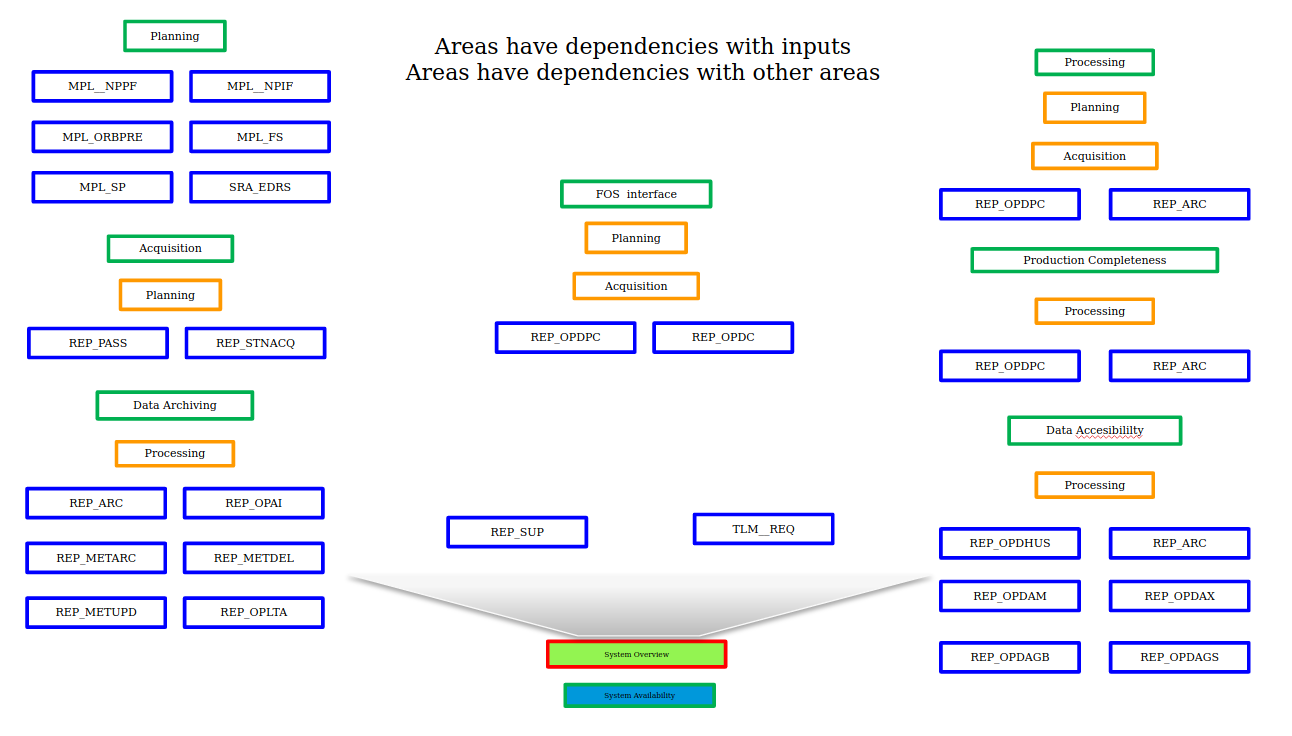
\includegraphics[width=150mm]{../fig/data_flow_s2boa.png}
	\caption{Areas of data related to the S2 mission}
	\label{fg:data_flow_s2boa}
  \end{center}
\end{figure}


This chapter describes each of the ingestion modules in the following sections. The figure \ref{fg:legened_structure_of_ingestions} shows the legend for the diagrams, used to represent the data stored.

\begin{figure}[H]
  \begin{center}
	\centering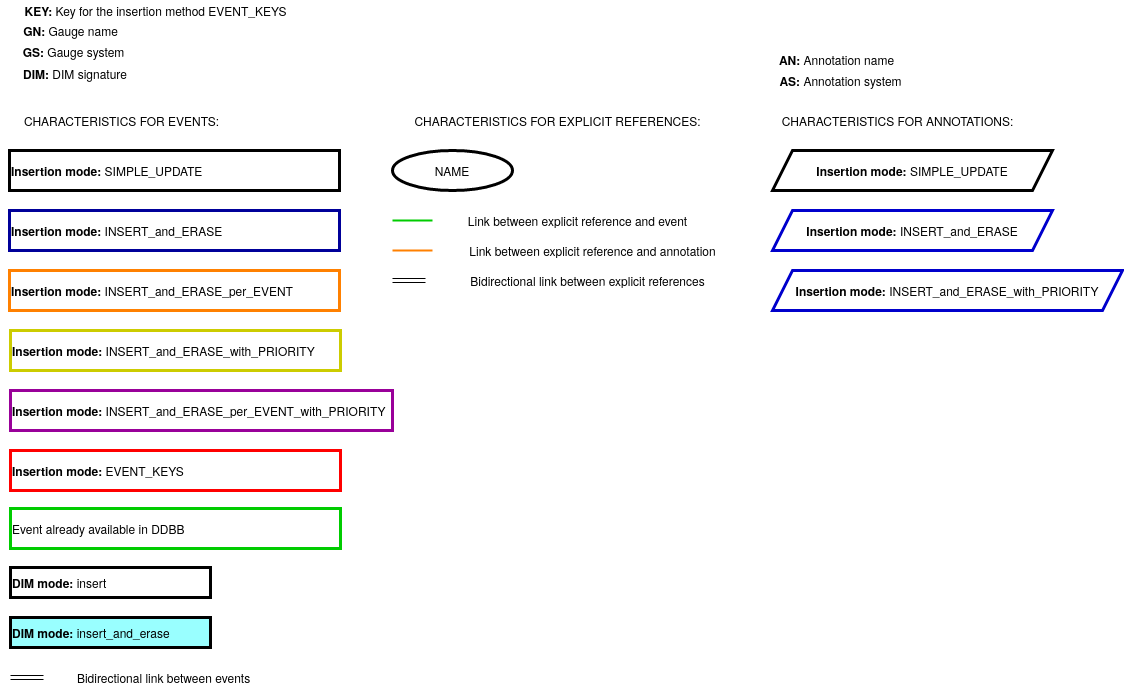
\includegraphics[width=150mm]{../fig/legened_structure_of_ingestions.png}
	\caption{Legend for the diagrams, used to represent the data stored}
	\label{fg:legened_structure_of_ingestions}
  \end{center}
\end{figure}

% Ingestion NPPF
\section{Ingestion module for the MPL\_NPPF file}

This sections describes the ingestion module for inserting the planning of operations commanding the satellite.

The associated ingestion processor is:

\begin{itemize} 

\item \textbf{s2boa.ingestions.ingestion\_nppf.ingestion\_nppf}
  
\end{itemize}

This module uses the following \acrshort{dim} signatures:

\begin{itemize} 

\item \textbf{NPPF\_XXX}: data corresponding to the planning of operations commanding the satellite.

\item \textbf{CORRECTED\_NPPF\_XXX}: data corresponding to the planning of operations commanding the satellite corrected by the available orbit prediction data.

\item \textbf{COMPLETENESS\_NPPF\_XXX}: data corresponding to the definition of planning completeness used for analysis.
  
\end{itemize}

Where XXX is the corresponding satellite id.

The figure \ref{fg:structure_ingestion_nppf} shows a simplified diagram of the structure of events inserted (associated structure of values not included for simplicity).

\begin{figure}[H]
  \begin{center}
	\centering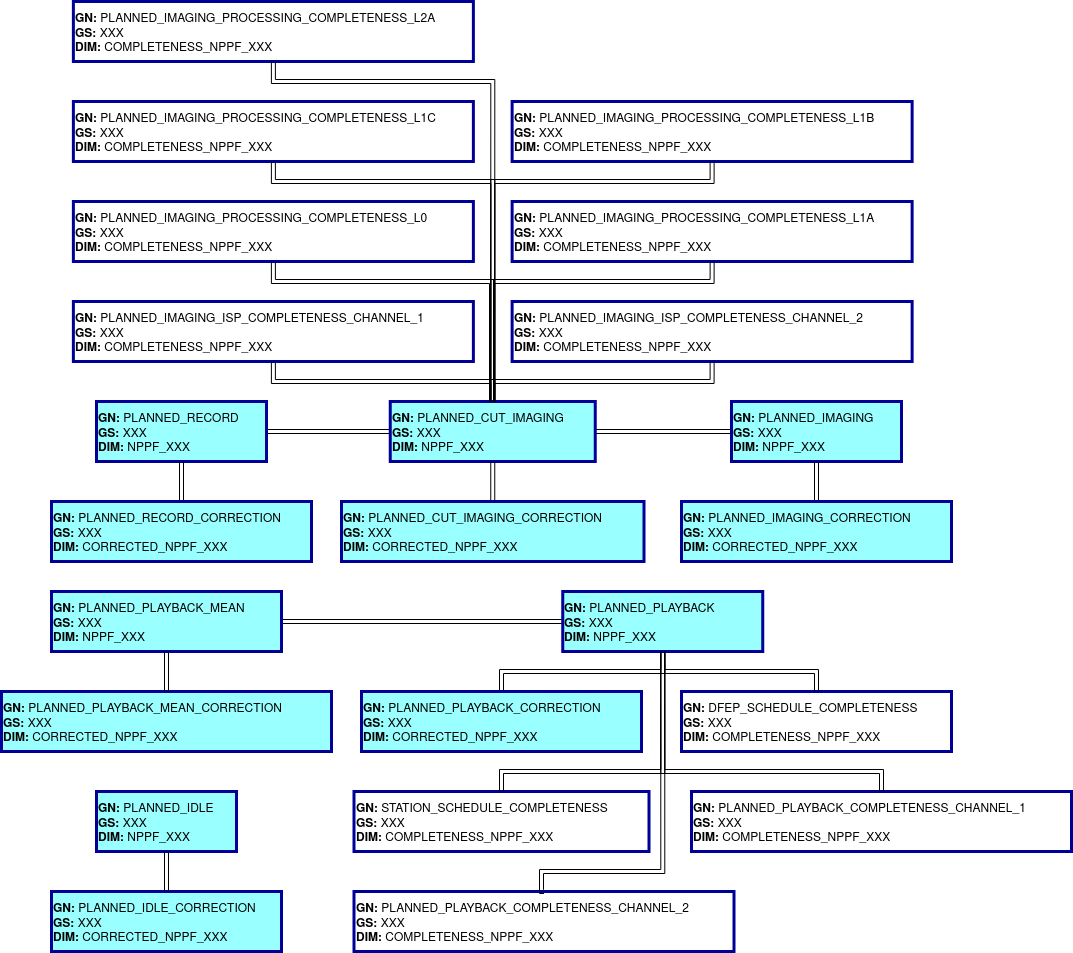
\includegraphics[width=150mm]{../fig/structure_ingestion_nppf.png}
	\caption{Structure of events inserted by the ingestion module for the MPL\_NPPF file}
	\label{fg:structure_ingestion_nppf}
  \end{center}
\end{figure}

The table \ref{tb:description_events_ingestion_nppf} shows the description of the events inserted by the ingestion.

\begin{landscape}
\begin{longtable}{|M{0.15\linewidth}|M{0.05\linewidth}|M{0.10\linewidth}|M{0.10\linewidth}|M{0.15\linewidth}|M{0.15\linewidth}|M{0.15\linewidth}|}
\hline \textbf{Gauge name} & \textbf{Gauge system} & \textbf{DIM signature} & \textbf{Insertion mode} & \textbf{Description} & \textbf{Start} & \textbf{Stop} \\ \hline
\textbf{PLANNED\_RECORD} & XXX & NPPF\_XXX & INSERT\_and\_ERASE (insert\_and\_erase) & Event for representing the \textbf{recording operation} & UTC time associated to command 'MPMMRNOM' or 'MPMMRNRT' & UTC time associated to command 'MPMMRSTP' or 'MPMMRNRT' or 'MPMMRNOM' \\ \hline
\textbf{PLANNED\_CUT\_IMAGING} & XXX & NPPF\_XXX & INSERT\_and\_ERASE (insert\_and\_erase) & Event for representing the \textbf{imaging operation associated to a specific recording operation} & UTC time associated to command 'MPMSSCAL' or 'MPMSDASC' or 'MPMSDCLO' or 'MPMSIVIC' or 'MPMSNOBS' or 'MPMSIRAW' or 'MPMSIDTS' or 'MPMMRNOM' or 'MPMMRNRT' & UTC time associated to command 'MPMSIMID' or 'MPMSIDSB' or 'MPMMRSTP' or 'MPMMRNRT' or 'MPMMRNOM' \\ \hline
\textbf{PLANNED\_IMAGING} & XXX & NPPF\_XXX & INSERT\_and\_ERASE (insert\_and\_erase) & Event for representing the \textbf{imaging operation} covering one or several planned recording operations & UTC time associated to command 'MPMSSCAL' or 'MPMSDASC' or 'MPMSDCLO' or 'MPMSIVIC' or 'MPMSNOBS' or 'MPMSIRAW' or 'MPMSIDTS' & UTC time associated to command 'MPMSIMID' or 'MPMSIDSB' or 'MPMMRSTP' \\ \hline
\textbf{PLANNED\_PLAYBACK} & XXX & NPPF\_XXX & INSERT\_and\_ERASE (insert\_and\_erase) & Event for representing the \textbf{playback operation} & UTC time associated to command 'MPMMPNOM' or 'MPMMPREG' or 'MPMMPBRT' or 'MPMMPNRT' & UTC time associated to command 'MPMMPSTP' \\ \hline
\textbf{PLANNED\_PLAYBACK\_MEAN} & XXX & NPPF\_XXX & INSERT\_and\_ERASE (insert\_and\_erase) & Event for representing the \textbf{mean of the playback operation} & UTC time associated to command 'MPXBSBOP' or 'MPG1STRT' or 'MPG2STRT' & UTC time associated to command 'MPXBOPSB' (when start is associated to command 'MPXBSBOP') or 'MPOCPRY2' (when start is associated to command 'MPG1STRT' or 'MPG2STRT') \\ \hline
\textbf{PLANNED\_IDLE} & XXX & NPPF\_XXX & INSERT\_and\_ERASE (insert\_and\_erase) & Event for representing the \textbf{idle state} & UTC time associated to command 'MPMSIMID' or 'MPMSSBID' & UTC time associated to command 'MPMSSCAL' or 'MPMSDASC' or 'MPMSDCLO' or 'MPMSIVIC' or 'MPMSNOBS' or 'MPMSIRAW' or 'MPMSIDTS' or 'MPMSIDSB' \\ \hline
\textbf{***\_CORRECTION} & XXX & \- CORRECTED\_NPPF\_XXX & INSERT\_and\_ERASE (insert\_and\_erase) & Event for representing the \textbf{planning events corrected using the orbit prediction events} & Start of the planned event corrected using the ORBPRE & Stop of the planned event corrected using the ORBPRE \\ \hline
\textbf{DFEP\_SCHEDULE\_COMPLETENESS} & XXX & \- COMPLETENESS & INSERT\_and\_ERASE (insert) & Event for representing the \textbf{expectation of the DFEP schedule} & Corrected start of the planned playback + 2s (SAD/HKTM) or + 9s (MSI); (if start \textgreater  stop) Corrected stop of the planned playback - 4s & Start (SAD/HKTM) or Corrected stop of the planned playback - 9s (MSI); (if start \textgreater  stop) Corrected stop of the planned playback - 3s \\ \hline
\textbf{STATION\_SCHEDULE\_COMPLETENESS} & XXX & \- COMPLETENESS\_NPPF\_XXX & INSERT\_and\_ERASE (insert) & Event for representing the \textbf{expectation of the Station schedule} & Corrected start of the planned playback + 2s (SAD/HKTM) or + 9s (MSI); (if start \textgreater  stop) Corrected stop of the planned playback - 4s & Start (SAD/HKTM) or Corrected stop of the planned playback - 9s (MSI); (if start \textgreater  stop) Corrected stop of the planned playback - 3s \\ \hline
\textbf{PLANNED\_PLAYBACK\_COMPLETENESS\_CHANNEL\_1} & XXX & \- COMPLETENESS\_NPPF\_XXX & INSERT\_and\_ERASE (insert) & Event for representing the \textbf{expectation of the planned playbacks using the channel 1} & Corrected start of the planned playback + 2s (SAD/HKTM) or + 9s (MSI); (if start \textgreater  stop) Corrected stop of the planned playback - 4s & Start (SAD/HKTM) or Corrected stop of the planned playback - 9s (MSI); (if start \textgreater  stop) Corrected stop of the planned playback - 3s \\ \hline
\textbf{PLANNED\_PLAYBACK\_COMPLETENESS\_CHANNEL\_2} & XXX & \- COMPLETENESS\_NPPF\_XXX & INSERT\_and\_ERASE (insert) & Event for representing the \textbf{expectation of the planned playbacks using the channel 2} & Corrected start of the planned playback + 2s (SAD/HKTM) or + 9s (MSI); (if start \textgreater  stop) Corrected stop of the planned playback - 4s & Start (SAD/HKTM) or Corrected stop of the planned playback - 9s (MSI); (if start \textgreater  stop) Corrected stop of the planned playback - 3s \\ \hline
\textbf{PLANNED\_IMAGING\_ISP\_COMPLETENESS\_CHANNEL\_1} & XXX & \- COMPLETENESS\_NPPF\_XXX & INSERT\_and\_ERASE (insert) & Event for representing the \textbf{expectation of the planned imaging using the channel 1} & Corrected start of the planned imaging + 10s; (if start \textgreater  stop) Corrected stop of the planned imaging - 12s & Corrected stop of the planned imaging - 10s; (if start \textgreater  stop) Corrected stop of the planned imaging - 6s \\ \hline
\textbf{PLANNED\_IMAGING\_ISP\_COMPLETENESS\_CHANNEL\_2} & XXX & \- COMPLETENESS\_NPPF\_XXX & INSERT\_and\_ERASE (insert) & Event for representing the \textbf{expectation of the planned imaging using the channel 2} & Corrected start of the planned imaging + 10s; (if start \textgreater  stop) Corrected stop of the planned imaging - 12s & Corrected stop of the planned imaging - 10s; (if start \textgreater  stop) Corrected stop of the planned imaging - 6s \\ \hline
\textbf{PLANNED\_IMAGING\_PROCESSING\_COMPLETENESS\_L0} & XXX & \- COMPLETENESS\_NPPF\_XXX & INSERT\_and\_ERASE (insert) & Event for representing the \textbf{expectation of the processing of the planned imaging for the L0} & Corrected start of the planned imaging + 10s; (if start \textgreater  stop) Corrected stop of the planned imaging - 12s & Corrected stop of the planned imaging - 10s; (if start \textgreater  stop) Corrected stop of the planned imaging - 6s \\ \hline
\textbf{PLANNED\_IMAGING\_PROCESSING\_COMPLETENESS\_L1A} & XXX & \- COMPLETENESS\_NPPF\_XXX & INSERT\_and\_ERASE (insert) & Event for representing the \textbf{expectation of the processing of the planned imaging for the L1A} & Corrected start of the planned imaging + 10s; (if start \textgreater  stop) Corrected stop of the planned imaging - 12s & Corrected stop of the planned imaging - 10s; (if start \textgreater  stop) Corrected stop of the planned imaging - 6s \\ \hline
\textbf{PLANNED\_IMAGING\_PROCESSING\_COMPLETENESS\_L1B} & XXX & \- COMPLETENESS\_NPPF\_XXX & INSERT\_and\_ERASE (insert) & Event for representing the \textbf{expectation of the processing of the planned imaging for the L1B} & Corrected start of the planned imaging + 10s; (if start \textgreater  stop) Corrected stop of the planned imaging - 12s & Corrected stop of the planned imaging - 10s; (if start \textgreater  stop) Corrected stop of the planned imaging - 6s \\ \hline
\textbf{PLANNED\_IMAGING\_PROCESSING\_COMPLETENESS\_L1C} & XXX & \- COMPLETENESS\_NPPF\_XXX & INSERT\_and\_ERASE (insert) & Event for representing the \textbf{expectation of the processing of the planned imaging for the L1C} & Corrected start of the planned imaging + 10s; (if start \textgreater  stop) Corrected stop of the planned imaging - 12s & Corrected stop of the planned imaging - 10s; (if start \textgreater  stop) Corrected stop of the planned imaging - 6s \\ \hline
\textbf{PLANNED\_IMAGING\_PROCESSING\_COMPLETENESS\_L2A} & XXX & \- COMPLETENESS\_NPPF\_XXX & INSERT\_and\_ERASE (insert) & Event for representing the \textbf{expectation of the processing of the planned imaging for the L2A} & Corrected start of the planned imaging + 10s; (if start \textgreater  stop) Corrected stop of the planned imaging - 12s & Corrected stop of the planned imaging - 10s; (if start \textgreater  stop) Corrected stop of the planned imaging - 6s \\ \hline
\caption{Table describing the events associated to the ingestion}
\label{tb:description_events_ingestion_nppf}
\end{longtable}
\end{landscape}

\subsection{Ingestion details}

This section describes some ingestion details for inserting the data. In particular:

\begin{itemize} 

\item The correction of the generation time when is greater than the validity start
  
\end{itemize}

\subsubsection{Correction of the generation time}

Due to an operation procedure using the \acrshort{s2mp}, the generation time could be greater than the validity start. This could result into having deprecated data in the DDBB.

To solve this issue the processor changes the generation time to be the validity start when the first is greater.


% Ingestion ORBPRE
\section{Ingestion module for the MPL\_ORBPRE file}

This sections describes the ingestion module for inserting the orbit prediction of the satellites generated by \acrshort{fos}.

The associated ingestion processor is:

\begin{itemize} 

\item \textbf{s2boa.ingestions.ingestion\_orbpre.ingestion\_orbpre}
  
\end{itemize}

This module uses the following \acrshort{dim} signatures:

\begin{itemize} 

\item \textbf{ORBPRE}: data corresponding to the orbit prediction of the satellites generated by \acrshort{fos} used for adjusting the timing of the planning events which are using the operations angle.

\item \textbf{CORRECTED\_NPPF\_XXX}: data corresponding to the planning of operations commanding the satellite corrected by the available orbit prediction data.

\item \textbf{COMPLETENESS\_NPPF\_XXX}: data corresponding to the definition of planning completeness used for analysis. \textbf{Priority is equal to 20}.
  
\end{itemize}

Where XXX is the corresponding satellite id.

The figure \ref{fg:structure_ingestion_orbpre} shows a simplified diagram of the structure of events inserted (associated structure of values not included for simplicity).

\begin{figure}[H]
  \begin{center}
	\centering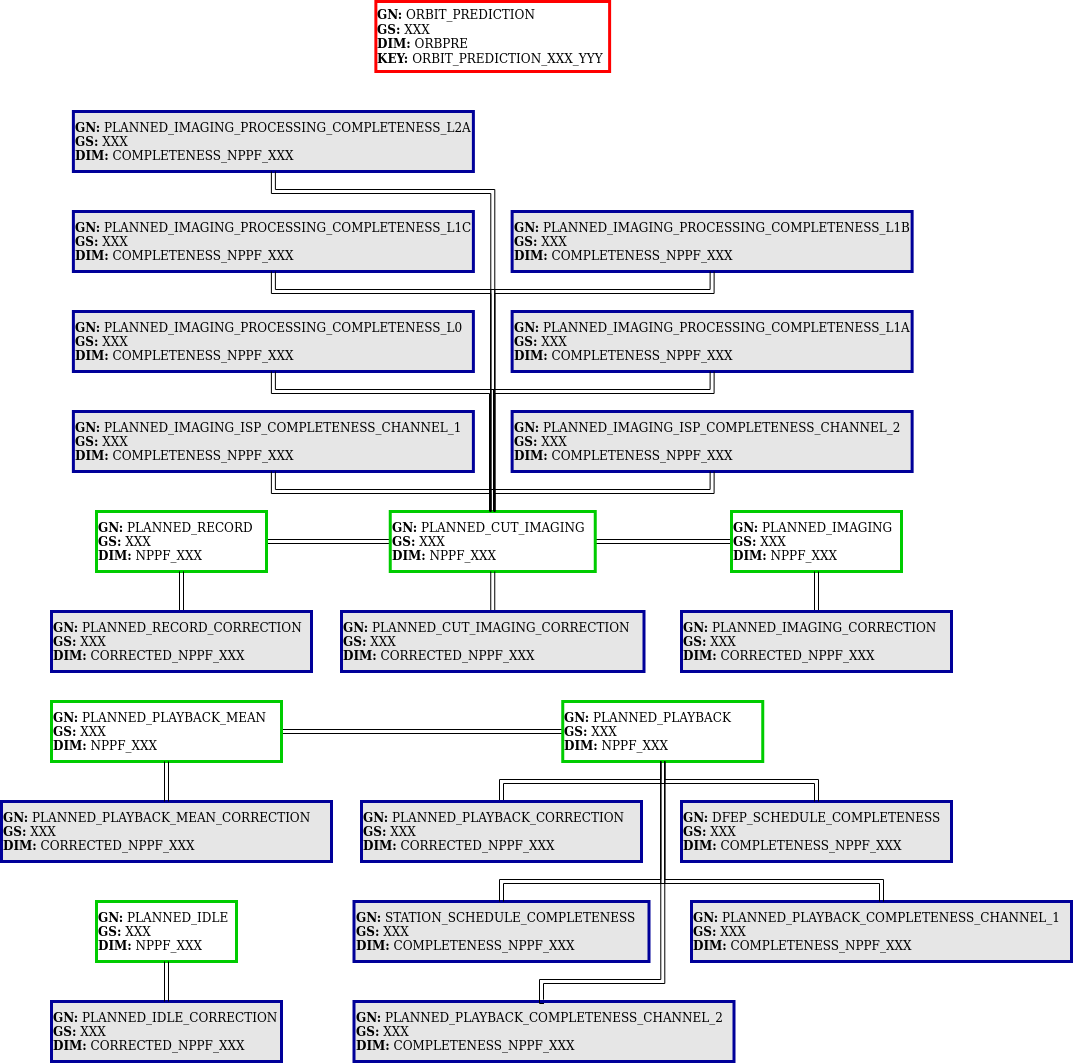
\includegraphics[width=150mm]{../fig/structure_ingestion_orbpre.png}
	\caption{Structure of events inserted by the ingestion module for the MPL\_ORBPRE file}
	\label{fg:structure_ingestion_orbpre}
  \end{center}
\end{figure}

Where YYY is the orbit number.

The table \ref{tb:description_events_ingestion_orbpre} shows the description of the events inserted by the ingestion.

\begin{landscape}
\begin{longtable}{|M{0.15\linewidth}|M{0.05\linewidth}|M{0.10\linewidth}|M{0.10\linewidth}|M{0.15\linewidth}|M{0.15\linewidth}|M{0.15\linewidth}|}
\hline \textbf{Gauge name} & \textbf{Gauge system} & \textbf{DIM signature} & \textbf{Insertion mode} & \textbf{Description} & \textbf{Start} & \textbf{Stop} \\ \hline
\textbf{ORBIT\_PREDICTION} & XXX & ORBIT\_PREDICTION\_XXX\_YYY & EVENT\_KEYS (insert) [KEY: ORBIT\_PREDICTION\_XXX\_YYY] & Event for representing the \textbf{orbit predition information of a specific orbit} & UTC time related to the ANX of orbit N & UTC time related to the ANX of orbit N + 1 \\ \hline
\textbf{***\_CORRECTION} & XXX & \- CORRECTED\_NPPF\_XXX & INSERT\_and\_ERASE (insert\_and\_erase) & Event for representing the \textbf{planning events corrected using the orbit prediction events} & Start of the planned event corrected using the ORBPRE & Stop of the planned event corrected using the ORBPRE \\ \hline
\textbf{DFEP\_SCHEDULE\_COMPLETENESS} & XXX & \- COMPLETENESS\_NPPF\_XXX & INSERT\_and\_ERASE\_with\_PRIORITY (insert) & Event for representing the \textbf{expectation of the DFEP schedule} & Corrected start of the planned playback + 2s (SAD/HKTM) or + 9s (MSI); (if start \textgreater  stop) Corrected stop of the planned playback - 4s & Start (SAD/HKTM) or Corrected stop of the planned playback - 9s (MSI); (if start \textgreater  stop) Corrected stop of the planned playback - 3s \\ \hline
\textbf{STATION\_SCHEDULE\_COMPLETENESS} & XXX & \- COMPLETENESS\_NPPF\_XXX & INSERT\_and\_ERASE\_with\_PRIORITY (insert) & Event for representing the \textbf{expectation of the Station schedule} & Corrected start of the planned playback + 2s (SAD/HKTM) or + 9s (MSI); (if start \textgreater  stop) Corrected stop of the planned playback - 4s & Start (SAD/HKTM) or Corrected stop of the planned playback - 9s (MSI); (if start \textgreater  stop) Corrected stop of the planned playback - 3s \\ \hline
\textbf{PLANNED\_PLAYBACK\_COMPLETENESS\_CHANNEL\_1} & XXX & \- COMPLETENESS\_NPPF\_XXX & INSERT\_and\_ERASE\_with\_PRIORITY (insert) & Event for representing the \textbf{expectation of the planned playbacks using the channel 1} & Corrected start of the planned playback + 2s (SAD/HKTM) or + 9s (MSI); (if start \textgreater  stop) Corrected stop of the planned playback - 4s & Start (SAD/HKTM) or Corrected stop of the planned playback - 9s (MSI); (if start \textgreater  stop) Corrected stop of the planned playback - 3s \\ \hline
\textbf{PLANNED\_PLAYBACK\_COMPLETENESS\_CHANNEL\_2} & XXX & \- COMPLETENESS\_NPPF\_XXX & INSERT\_and\_ERASE\_with\_PRIORITY (insert) & Event for representing the \textbf{expectation of the planned playbacks using the channel 2} & Corrected start of the planned playback + 2s (SAD/HKTM) or + 9s (MSI); (if start \textgreater  stop) Corrected stop of the planned playback - 4s & Start (SAD/HKTM) or Corrected stop of the planned playback - 9s (MSI); (if start \textgreater  stop) Corrected stop of the planned playback - 3s \\ \hline
\textbf{PLANNED\_IMAGING\_ISP\_COMPLETENESS\_CHANNEL\_1} & XXX & \- COMPLETENESS\_NPPF\_XXX & INSERT\_and\_ERASE\_with\_PRIORITY (insert) & Event for representing the \textbf{expectation of the planned imaging using the channel 1} & Corrected start of the planned imaging + 10s; (if start \textgreater  stop) Corrected stop of the planned imaging - 12s & Corrected stop of the planned imaging - 10s; (if start \textgreater  stop) Corrected stop of the planned imaging - 6s \\ \hline
\textbf{PLANNED\_IMAGING\_ISP\_COMPLETENESS\_CHANNEL\_2} & XXX & \- COMPLETENESS\_NPPF\_XXX & INSERT\_and\_ERASE\_with\_PRIORITY (insert) & Event for representing the \textbf{expectation of the planned imaging using the channel 2} & Corrected start of the planned imaging + 10s; (if start \textgreater  stop) Corrected stop of the planned imaging - 12s & Corrected stop of the planned imaging - 10s; (if start \textgreater  stop) Corrected stop of the planned imaging - 6s \\ \hline
\textbf{PLANNED\_IMAGING\_PROCESSING\_COMPLETENESS\_L0} & XXX & \- COMPLETENESS\_NPPF\_XXX & INSERT\_and\_ERASE\_with\_PRIORITY (insert) & Event for representing the \textbf{expectation of the processing of the planned imaging for the L0} & Corrected start of the planned imaging + 10s; (if start \textgreater  stop) Corrected stop of the planned imaging - 12s & Corrected stop of the planned imaging - 10s; (if start \textgreater  stop) Corrected stop of the planned imaging - 6s \\ \hline
\textbf{PLANNED\_IMAGING\_PROCESSING\_COMPLETENESS\_L1A} & XXX & \- COMPLETENESS\_NPPF\_XXX & INSERT\_and\_ERASE\_with\_PRIORITY (insert) & Event for representing the \textbf{expectation of the processing of the planned imaging for the L1A} & Corrected start of the planned imaging + 10s; (if start \textgreater  stop) Corrected stop of the planned imaging - 12s & Corrected stop of the planned imaging - 10s; (if start \textgreater  stop) Corrected stop of the planned imaging - 6s \\ \hline
\textbf{PLANNED\_IMAGING\_PROCESSING\_COMPLETENESS\_L1B} & XXX & \- COMPLETENESS\_NPPF\_XXX & INSERT\_and\_ERASE\_with\_PRIORITY (insert) & Event for representing the \textbf{expectation of the processing of the planned imaging for the L1B} & Corrected start of the planned imaging + 10s; (if start \textgreater  stop) Corrected stop of the planned imaging - 12s & Corrected stop of the planned imaging - 10s; (if start \textgreater  stop) Corrected stop of the planned imaging - 6s \\ \hline
\textbf{PLANNED\_IMAGING\_PROCESSING\_COMPLETENESS\_L1C} & XXX & \- COMPLETENESS\_NPPF\_XXX & INSERT\_and\_ERASE\_with\_PRIORITY (insert) & Event for representing the \textbf{expectation of the processing of the planned imaging for the L1C} & Corrected start of the planned imaging + 10s; (if start \textgreater  stop) Corrected stop of the planned imaging - 12s & Corrected stop of the planned imaging - 10s; (if start \textgreater  stop) Corrected stop of the planned imaging - 6s \\ \hline
\textbf{PLANNED\_IMAGING\_PROCESSING\_COMPLETENESS\_L2A} & XXX & \- COMPLETENESS\_NPPF\_XXX & INSERT\_and\_ERASE\_with\_PRIORITY (insert) & Event for representing the \textbf{expectation of the processing of the planned imaging for the L2A} & Corrected start of the planned imaging + 10s; (if start \textgreater  stop) Corrected stop of the planned imaging - 12s & Corrected stop of the planned imaging - 10s; (if start \textgreater  stop) Corrected stop of the planned imaging - 6s \\ \hline
\caption{Table describing the events associated to the ingestion}
\label{tb:description_events_ingestion_orbpre}
\end{longtable}
\end{landscape}

\subsection{Ingestion details}

This section describes some ingestion details for inserting the data. In particular:

\begin{itemize} 

\item The algorithm to correct the timing of the planning events

\item The correction of the generation time to avoid overriding data used for completeness analysis
  
\end{itemize}

\subsubsection{Algorithm to correct the timing of the planning events}

The algorithm to correct the timing of the planning events is as follows:

For every planning event:

\begin{itemize} 

\item Get satellite ID, start and stop orbits and start and stop angles.

\item Get the \acrshort{anx} time from the orbit prediction information covering the previous orbits and the following ones

\item Apply the following formula to the start and stop angles (\(\alpha\)) using the orbital period (p) and the corresponding \acrshort{anx} timing (t):

  \(sin_1 = sin(\alpha)\)

  \(sin_2 = sin(2*\alpha)\)

  \(cos_1 = cos(\alpha)\)

  \(cos_2 = cos(2*\alpha)\)

  \(cos_3 = cos(3*\alpha)\)

  Adjust angle to a circunference (perfect distribution in 360º):
  
  \(m = \alpha - 0.13175612 - 2*(-0.0001529)*sin_1 - 2*(-0.0660818)*cos_1 - 2*0.16855853*sin_2 - 2*(-0.0007759)*cos_2 - 2*0.0009872*cos_3 - 2*0.00687159*sin_2\)

  Transform angle to \(\delta\) time:
  
  \(s = (m * p)/360.0\)

  \(UTC time = t + s \)
  
\end{itemize}

\subsubsection{Correction of the generation time}

The validity start of the ORBPRE is almost equal to the generation time. This makes the data extracted to be in priority with respect to the data extracted of other components which would need to be in priority.

To solve this issue the processor changes the generation time to be the generation time minus 1 day.


% Ingestion MPL_SP
\section{Ingestion module for the MPL\_SP file}

This sections describes the ingestion module for inserting the station schedule information received from the S2 Mission Planning.

The associated ingestion processors are:

\begin{itemize} 

\item \textbf{s2boa.ingestions.ingestion\_station\_schedule.ingestion\_station\_schedule}
  
\end{itemize}

This module uses the following \acrshort{dim} signatures:

\begin{itemize} 

\item \textbf{STATION\_SCHEDULE\_WWW\_XXX}: data corresponding to station schedule information associated to a specific station and satellite received from the Mission Planning.

\item \textbf{COMPLETENESS\_NPPF\_XXX}: data corresponding to the definition of planning completeness used for analysis.
  
\end{itemize}

Where XXX is the corresponding satellite id and WWW to the station ID.

The figure \ref{fg:structure_ingestion_station_schedule} shows a simplified diagram of the structure of events inserted (associated structure of values not included for simplicity).

\begin{figure}[H]
  \begin{center}
	\centering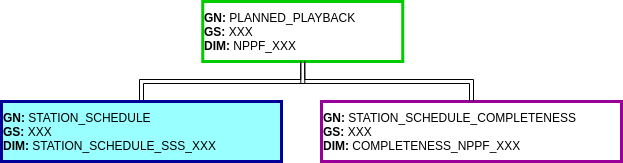
\includegraphics[width=150mm]{structure_ingestion_station_schedule.png}
	\caption{Structure of events inserted by the ingestion module for the MPL\_SP file}
	\label{fg:structure_ingestion_station_schedule}
  \end{center}
\end{figure}

The table \ref{tb:description_events_ingestion_station_schedule} shows the description of the events inserted by the ingestion.

\begin{landscape}
\begin{longtable}{|M{0.15\linewidth}|M{0.05\linewidth}|M{0.10\linewidth}|M{0.10\linewidth}|M{0.15\linewidth}|M{0.15\linewidth}|M{0.15\linewidth}|}
\hline \textbf{Gauge name} & \textbf{Gauge system} & \textbf{DIM signature} & \textbf{Insertion mode} & \textbf{Description} & \textbf{Start} & \textbf{Stop} \\ \hline
\textbf{STATION\_SCHEDULE} & XXX & STATION\_SCHEDULE\_WWW\_XXX & ERASE\_and\_REPLACE\_per\_EVENT (insert) & Event for representing the \textbf{station schedule} & UTC value inside the Data\_start node & UTC value inside the Data\_stop node  \\ \hline
\textbf{STATION\_SCHEDULE\_COMPLETENESS} & XXX & \- COMPLETENESS\_NPPF\_XXX & ERASE\_and\_REPLACE (insert\_and\_erase) & Event for representing the \textbf{expectation of the Station schedule} & UTC value inside the Data\_start node & UTC value inside the Data\_stop node  \\ \hline
\caption{Table describing the events associated to the ingestion}
\label{tb:description_events_ingestion_station_schedule}
\end{longtable}
\end{landscape}

\subsection{Ingestion details}

This section describes some ingestion details for inserting the data. In particular:

\begin{itemize} 

\item The correction of the generation time to avoid overriding data used for completeness analysis
  
\end{itemize}

\subsubsection{Correction of the generation time}

The generation time of the data extracted is one day before the validity start. This could be a problem as the processor of the ORBPRE files could override this data.

To solve this issue the processor changes the generation time to be the validity start.


% Ingestion MPL_FS
\section{Ingestion module for the MPL\_FS file}

This sections describes the ingestion module for inserting the DFEP schedule information received from the S2 Mission Planning.

The associated ingestion processor is:

\begin{itemize} 

\item \textbf{s2boa.ingestions.ingestion\_dfep\_schedule.ingestion\_dfep\_schedule}
  
\end{itemize}

This module uses the following \acrshort{dim} signatures:

\begin{itemize} 

\item \textbf{DFEP\_SCHEDULE\_WWW\_XXX}: data corresponding to DFEP schedule information associated to a specific station and satellite received from the Mission Planning.

\item \textbf{COMPLETENESS\_NPPF\_XXX}: data corresponding to the definition of planning completeness used for analysis. \textbf{Priority is equal to 30}.
  
\end{itemize}

Where XXX is the corresponding satellite id and WWW to the station ID.

The figure \ref{fg:structure_ingestion_dfep_schedule} shows a simplified diagram of the structure of events inserted (associated structure of values not included for simplicity).

\begin{figure}[H]
  \begin{center}
	\centering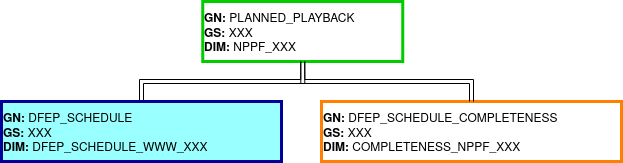
\includegraphics[width=150mm]{../fig/structure_ingestion_dfep_schedule.png}
	\caption{Structure of events inserted by the ingestion module for the MPL\_FS file}
	\label{fg:structure_ingestion_dfep_schedule}
  \end{center}
\end{figure}

The table \ref{tb:description_events_ingestion_dfep_schedule} shows the description of the events inserted by the ingestion.

\begin{landscape}
\begin{longtable}{|M{0.15\linewidth}|M{0.05\linewidth}|M{0.10\linewidth}|M{0.10\linewidth}|M{0.15\linewidth}|M{0.15\linewidth}|M{0.15\linewidth}|}
\hline \textbf{Gauge name} & \textbf{Gauge system} & \textbf{DIM signature} & \textbf{Insertion mode} & \textbf{Description} & \textbf{Start} & \textbf{Stop} \\ \hline
\textbf{DFEP\_SCHEDULE} & XXX & DFEP\_SCHEDULE\_WWW\_XXX & INSERT\_and\_ERASE\_per\_EVENT\_with\_PRIORITY (insert) & Event for representing the \textbf{DFEP schedule} & UTC value inside the start node & UTC value inside the stop node \\ \hline
\textbf{DFEP\_SCHEDULE\_COMPLETENESS} & XXX & \- COMPLETENESS\_NPPF\_XXX & INSERT\_and\_ERASE & Event for representing the \textbf{expectation of the DFEP schedule} & UTC value inside the start node & UTC value inside the stop node \\ \hline
\caption{Table describing the events associated to the ingestion}
\label{tb:description_events_ingestion_dfep_schedule}
\end{longtable}
\end{landscape}

\subsection{Ingestion details}

This section describes some ingestion details for inserting the data. In particular:

\begin{itemize} 

\item The correction of the generation time to avoid overriding data used for completeness analysis
  
\end{itemize}

\subsubsection{Correction of the generation time}

The generation time of the data extracted is one day before the validity start. This could be a problem as the processor of the ORBPRE files could override this data.

To solve this issue the processor changes the generation time to be the validity start.


% Ingestion SRA
\section{Ingestion module for the SRA file}

This sections describes the ingestion module for inserting the SRA information received from the \acrshort{edrs}.

The associated ingestion processor is:

\begin{itemize} 

\item \textbf{s2boa.ingestions.ingestion\_slot\_request\_edrs.ingestion\_slot\_request\_edrs}
  
\end{itemize}

This module uses the following \acrshort{dim} signatures:

\begin{itemize} 

\item \textbf{SLOT\_REQUEST\_EDRS}: data corresponding to the slot request information associated to the EDRS service.

\item \textbf{COMPLETENESS\_NPPF\_XXX}: data corresponding to the definition of planning completeness used for analysis.
  
\end{itemize}

Where XXX is the corresponding satellite ID.

The figure \ref{fg:structure_ingestion_slot_request_edrs} shows a simplified diagram of the structure of events inserted (associated structure of values not included for simplicity).

\begin{figure}[H]
  \begin{center}
	\centering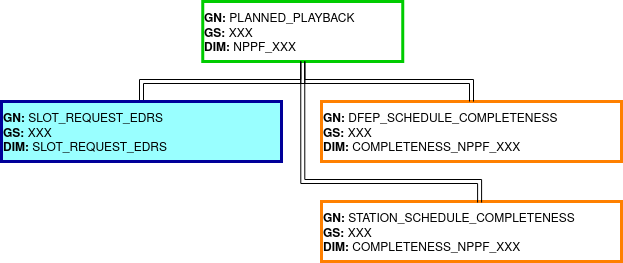
\includegraphics[width=150mm]{../fig/structure_ingestion_slot_request_edrs.png}
	\caption{Structure of events inserted by the ingestion module for the SRA file}
	\label{fg:structure_ingestion_slot_request_edrs}
  \end{center}
\end{figure}

The table \ref{tb:description_events_ingestion_slot_request_edrs} shows the description of the events inserted by the ingestion.

\begin{landscape}
\begin{longtable}{|M{0.15\linewidth}|M{0.05\linewidth}|M{0.10\linewidth}|M{0.10\linewidth}|M{0.15\linewidth}|M{0.15\linewidth}|M{0.15\linewidth}|}
\hline \textbf{Gauge name} & \textbf{Gauge system} & \textbf{DIM signature} & \textbf{Insertion mode} & \textbf{Description} & \textbf{Start} & \textbf{Stop} \\ \hline
\textbf{SLOT\_REQUEST\_EDRS} & XXX & SLOT\_REQUEST\_EDRS & ERASE\_and\_REPLACE\_per\_EVENT (insert) & Event for representing the \textbf{slot request for \acrshort{edrs}} & UTC value inside the Start\_Time node & UTC value inside the Stop\_Time node \\ \hline
\textbf{STATION\_SCHEDULE\_COMPLETENESS} & XXX & \- COMPLETENESS\_NPPF\_XXX & ERASE\_and\_REPLACE (insert\_and\_erase) & Event for representing the \textbf{expectation of the Station schedule} & UTC value inside the Start\_Time node & UTC value inside the Stop\_Time node \\ \hline
\textbf{DFEP\_SCHEDULE\_COMPLETENESS} & XXX & \- COMPLETENESS\_NPPF\_XXX & ERASE\_and\_REPLACE (insert\_and\_erase) & Event for representing the \textbf{expectation of the DFEP schedule} & UTC value inside the Start\_Time node & UTC value inside the Stop\_Time node \\ \hline
\caption{Table describing the events associated to the ingestion}
\label{tb:description_events_ingestion_slot_request_edrs}
\end{longtable}
\end{landscape}


% Ingestion of the REP_PASS_[2|5]
\section{Ingestion module for the REP\_PASS\_[2|5] file}

This sections describes the ingestion module for inserting the \acrshort{dfep} acquisition analysis after reception of data from the satellite.

The associated ingestion processor is:

\begin{itemize} 

\item \textbf{s2boa.ingestions.ingestion\_dfep\_acquisition.ingestion\_dfep\_acquisition}
  
\end{itemize}

This module uses the following \acrshort{dim} signatures:

\begin{itemize} 

\item \textbf{RECEPTION\_XXX}: data corresponding to the acquisition analysis after reception of data from the satellite.

\item \textbf{COMPLETENESS\_NPPF\_XXX}: data corresponding to the definition of planning completeness used for analysis. \textbf{Priority is equal to 30}.

\item \textbf{ISP\_VALIDITY\_PROCESSING\_COMPLETENESS\_XXX}: data corresponding to the definition of \acrshort{isp} processing completeness used for analysis. \textbf{Priority is equal to 10}.

\end{itemize}

Where XXX is the corresponding satellite id, SSS is the station ID and VVV is the \acrshort{vcid} number.

The figure \ref{fg:structure_ingestion_dfep_acquisition} shows a simplified diagram of the structure of events inserted (associated structure of values not included for simplicity).

\begin{figure}[H]
  \begin{center}
	\centering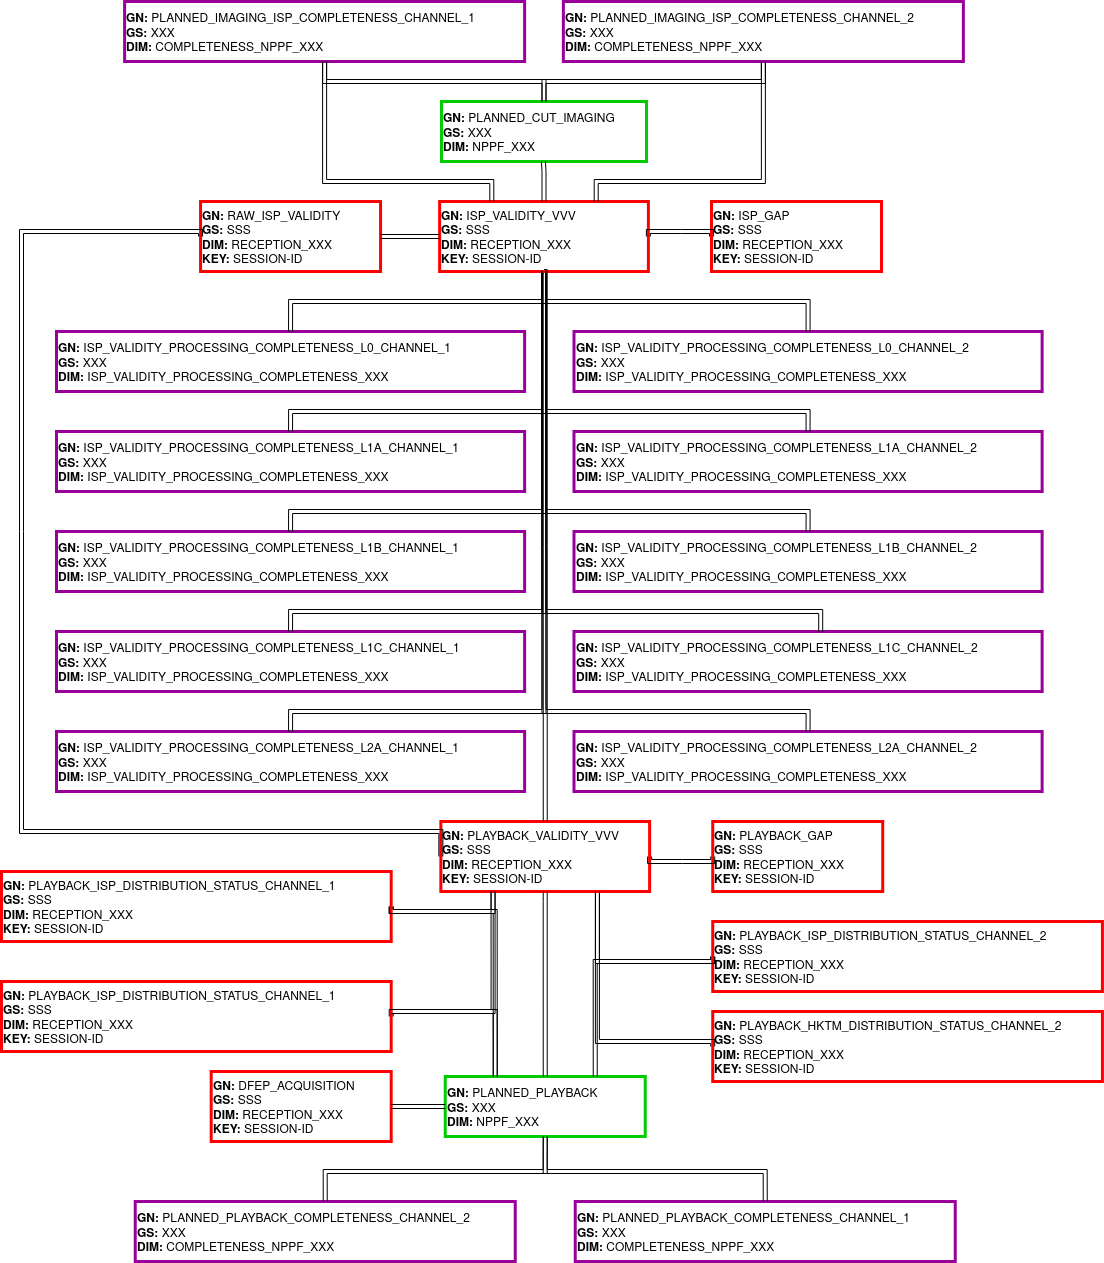
\includegraphics[width=150mm]{../fig/structure_ingestion_dfep_acquisition.png}
	\caption{Structure of events inserted by the ingestion module for the REP\_PASS\_[2|5] file}
	\label{fg:structure_ingestion_dfep_acquisition}
  \end{center}
\end{figure}

The table \ref{tb:description_events_ingestion_dfep_acquisition} shows the description of the events inserted by the ingestion.

\begin{landscape}
\begin{longtable}{|M{0.15\linewidth}|M{0.05\linewidth}|M{0.10\linewidth}|M{0.10\linewidth}|M{0.15\linewidth}|M{0.15\linewidth}|M{0.15\linewidth}|}
\hline \textbf{Gauge name} & \textbf{Gauge system} & \textbf{DIM signature} & \textbf{Insertion mode} & \textbf{Description} & \textbf{Start} & \textbf{Stop} \\ \hline
\textbf{PLAYBACK\_VALIDITY\_VVV} & SSS & \- RECEPTION\_XXX & EVENT\_KEYS (insert) [KEY: SESSION-ID] & Event for representing the \textbf{ground acquisition operation} & UTC time associated to the start of the reception & UTC time associated to the stop of the reception \\ \hline
\textbf{PLAYBACK\_GAP} & SSS & \- RECEPTION\_XXX & EVENT\_KEYS (insert) [KEY: SESSION-ID] & Event for representing a \textbf{gap in the ground acquisition operation} & UTC time associated to the start of the corresponding gap in the reception & UTC time associated to the stop of the corresponding gap in the reception \\ \hline
\textbf{PLANNED\_PLAYBACK\_COMPLETENESS\_CHANNEL\_1} & XXX & \- COMPLETENESS\_NPPF\_XXX & INSERT\_and\_ERASE\_per\_EVENT\_with\_PRIORITY (insert) & Event for completing the \textbf{expectation of the planned playbacks through the channel 1} & Start of the reception through the channel 1 & Stop of the reception through the channel 1 \\ \hline
\textbf{PLANNED\_PLAYBACK\_COMPLETENESS\_CHANNEL\_2} & XXX & \- COMPLETENESS\_NPPF\_XXX & INSERT\_and\_ERASE\_per\_EVENT\_with\_PRIORITY (insert) & Event for completing the \textbf{expectation of the planned playbacks through the channel 2} & Start of the reception through the channel 2 & Stop of the reception through the channel 2 \\ \hline
\textbf{PLANNED\_IMAGING\_ISP\_COMPLETENESS\_CHANNEL\_1} & XXX & \- COMPLETENESS\_NPPF\_XXX & INSERT\_and\_ERASE\_per\_EVENT\_with\_PRIORITY (insert) & Event for completing the \textbf{expectation of the planned imaging sent through the channel 1} & Start of the first received scene thorugh the channel 1 of the corresponding continuous \acrshort{msi} segment & Stop of the last received scene thorugh the channel 1 of the corresponding continuous \acrshort{msi} segment \\ \hline
\textbf{PLANNED\_IMAGING\_ISP\_COMPLETENESS\_CHANNEL\_2} & XXX & \- COMPLETENESS\_NPPF\_XXX & INSERT\_and\_ERASE\_per\_EVENT\_with\_PRIORITY (insert) & Event for completing the \textbf{expectation of the planned imaging sent through the channel 2} & Start of the first received scene thorugh the channel 2 of the corresponding continuous \acrshort{msi} segment & Stop of the last received scene thorugh the channel 2 of the corresponding continuous \acrshort{msi} segment \\ \hline
\textbf{RAW\_ISP\_VALIDITY} & SSS & \- RECEPTION\_XXX & EVENT\_KEYS (insert) [KEY: SESSION-ID] & Event for representing the \textbf{ground acquisition operation} & Start of the first received scene & Stop of the last received scene \\ \hline
\textbf{ISP\_VALIDITY} & SSS & \- RECEPTION\_XXX & EVENT\_KEYS (insert) [KEY: SESSION-ID] & Event for representing the \textbf{ground acquisition operation} & Start of the first received scene of the corresponding continuous \acrshort{msi} segment & Stop of the last received scene of the corresponding continuous \acrshort{msi} segment \\ \hline
\textbf{ISP\_GAP} & SSS & \- RECEPTION\_XXX & EVENT\_KEYS (insert) [KEY: SESSION-ID] & Event for representing a \textbf{gap in the ground acquisition operation} & UTC time associated to the start of the corresponding continuous gap in the received MSI & UTC time associated to the stop of the corresponding continuous gap in the received MSI \\ \hline
\textbf{PLAYBACK\_ISP\_DISTRIBUTION\_STATUS\_CHANNEL\_1} & SSS & \- RECEPTION\_XXX & EVENT\_KEYS (insert) [KEY: SESSION-ID] & Event for representing a \textbf{gap in the ground acquisition operation} & UTC time associated to the start of the \acrshort{msi} reception & UTC time associated to the stop of the \acrshort{msi} reception \\ \hline
\textbf{PLAYBACK\_ISP\_DISTRIBUTION\_STATUS\_CHANNEL\_2} & SSS & \- RECEPTION\_XXX & EVENT\_KEYS (insert) [KEY: SESSION-ID] & Event for representing a \textbf{gap in the ground acquisition operation} & UTC time associated to the start of the \acrshort{msi} reception & UTC time associated to the stop of the \acrshort{msi} reception \\ \hline
\textbf{PLAYBACK\_HKTM\_DISTRIBUTION\_STATUS\_CHANNEL\_1} & SSS & \- RECEPTION\_XXX & EVENT\_KEYS (insert) [KEY: SESSION-ID] & Event for representing a \textbf{gap in the ground acquisition operation} & UTC time associated to the start of the corresponding gap in the \acrshort{hktm} reception & UTC time associated to the stop of the corresponding gap in the \acrshort{hktm} reception \\ \hline
\textbf{PLAYBACK\_HKTM\_DISTRIBUTION\_STATUS\_CHANNEL\_2} & SSS & \- RECEPTION\_XXX & EVENT\_KEYS (insert) [KEY: SESSION-ID] & Event for representing a \textbf{gap in the ground acquisition operation} & UTC time associated to the start of the corresponding gap in the \acrshort{hktm} reception & UTC time associated to the stop of the corresponding gap in the \acrshort{hktm} reception \\ \hline
\textbf{DFEP\_ACQUISITION\_VALIDITY} & SSS & \- RECEPTION\_XXX & EVENT\_KEYS (insert) [KEY: SESSION-ID] & Event for representing a \textbf{gap in the ground acquisition operation} & UTC time associated to the validity start of the received file & UTC time associated to the validity stop of the received file \\ \hline
\textbf{ISP\_VALIDITY\_PROCESSING\_COMPLETENESS\_L0\_CHANNEL\_1} & XXX & \- COMPLETENESS\_NPPF\_XXX & INSERT\_and\_ERASE\_per\_EVENT\_with\_PRIORITY (insert) & Event for representing the \textbf{expectation of the processing of the planned imaging for the L0} & Start of the first received scene of the corresponding continuous \acrshort{msi} segment & Stop of the last received scene of the corresponding continuous \acrshort{msi} segment \\ \hline
\textbf{ISP\_VALIDITY\_PROCESSING\_COMPLETENESS\_L1A\_CHANNEL\_1} & XXX & \- COMPLETENESS\_NPPF\_XXX & INSERT\_and\_ERASE\_per\_EVENT\_with\_PRIORITY (insert) & Event for representing the \textbf{expectation of the processing of the planned imaging for the L0} & Start of the first received scene of the corresponding continuous \acrshort{msi} segment & Stop of the last received scene of the corresponding continuous \acrshort{msi} segment \\ \hline
\textbf{ISP\_VALIDITY\_PROCESSING\_COMPLETENESS\_L1B\_CHANNEL\_1} & XXX & \- COMPLETENESS\_NPPF\_XXX & INSERT\_and\_ERASE\_per\_EVENT\_with\_PRIORITY (insert) & Event for representing the \textbf{expectation of the processing of the planned imaging for the L0} & Start of the first received scene of the corresponding continuous \acrshort{msi} segment & Stop of the last received scene of the corresponding continuous \acrshort{msi} segment \\ \hline
\textbf{ISP\_VALIDITY\_PROCESSING\_COMPLETENESS\_L1C\_CHANNEL\_1} & XXX & \- COMPLETENESS\_NPPF\_XXX & INSERT\_and\_ERASE\_per\_EVENT\_with\_PRIORITY (insert) & Event for representing the \textbf{expectation of the processing of the planned imaging for the L0} & Start of the first received scene of the corresponding continuous \acrshort{msi} segment & Stop of the last received scene of the corresponding continuous \acrshort{msi} segment \\ \hline
\textbf{ISP\_VALIDITY\_PROCESSING\_COMPLETENESS\_L2A\_CHANNEL\_1} & XXX & \- COMPLETENESS\_NPPF\_XXX & INSERT\_and\_ERASE\_per\_EVENT\_with\_PRIORITY (insert) & Event for representing the \textbf{expectation of the processing of the planned imaging for the L0} & Start of the first received scene of the corresponding continuous \acrshort{msi} segment & Stop of the last received scene of the corresponding continuous \acrshort{msi} segment \\ \hline
\textbf{ISP\_VALIDITY\_PROCESSING\_COMPLETENESS\_L0\_CHANNEL\_2} & XXX & \- COMPLETENESS\_NPPF\_XXX & INSERT\_and\_ERASE\_per\_EVENT\_with\_PRIORITY (insert) & Event for representing the \textbf{expectation of the processing of the planned imaging for the L0} & Start of the first received scene of the corresponding continuous \acrshort{msi} segment & Stop of the last received scene of the corresponding continuous \acrshort{msi} segment \\ \hline
\textbf{ISP\_VALIDITY\_PROCESSING\_COMPLETENESS\_L1A\_CHANNEL\_2} & XXX & \- COMPLETENESS\_NPPF\_XXX & INSERT\_and\_ERASE\_per\_EVENT\_with\_PRIORITY (insert) & Event for representing the \textbf{expectation of the processing of the planned imaging for the L0} & Start of the first received scene of the corresponding continuous \acrshort{msi} segment & Stop of the last received scene of the corresponding continuous \acrshort{msi} segment \\ \hline
\textbf{ISP\_VALIDITY\_PROCESSING\_COMPLETENESS\_L1B\_CHANNEL\_2} & XXX & \- COMPLETENESS\_NPPF\_XXX & INSERT\_and\_ERASE\_per\_EVENT\_with\_PRIORITY (insert) & Event for representing the \textbf{expectation of the processing of the planned imaging for the L0} & Start of the first received scene of the corresponding continuous \acrshort{msi} segment & Stop of the last received scene of the corresponding continuous \acrshort{msi} segment \\ \hline
\textbf{ISP\_VALIDITY\_PROCESSING\_COMPLETENESS\_L1C\_CHANNEL\_2} & XXX & \- COMPLETENESS\_NPPF\_XXX & INSERT\_and\_ERASE\_per\_EVENT\_with\_PRIORITY (insert) & Event for representing the \textbf{expectation of the processing of the planned imaging for the L0} & Start of the first received scene of the corresponding continuous \acrshort{msi} segment & Stop of the last received scene of the corresponding continuous \acrshort{msi} segment \\ \hline
\textbf{ISP\_VALIDITY\_PROCESSING\_COMPLETENESS\_L2A\_CHANNEL\_2} & XXX & \- COMPLETENESS\_NPPF\_XXX & INSERT\_and\_ERASE\_per\_EVENT\_with\_PRIORITY (insert) & Event for representing the \textbf{expectation of the processing of the planned imaging for the L0} & Start of the first received scene of the corresponding continuous \acrshort{msi} segment & Stop of the last received scene of the corresponding continuous \acrshort{msi} segment \\ \hline
\caption{Table describing the events associated to the ingestion}
\label{tb:description_events_ingestion_dfep_acquisition}
\end{longtable}
\end{landscape}


% Ingestion of the REP_PASS_E
\section{Ingestion module for the REP\_PASS\_E file}

This sections describes the ingestion module for inserting the \acrshort{efep} acquisition analysis after reception of data from the satellite.

The associated ingestion processor is:

\begin{itemize} 

\item \textbf{s2boa.ingestions.ingestion\_edrs\_acquisition.ingestion\_edrs\_acquisition}

\item \textbf{s2boa.ingestions.ingestion\_vgs\_acquisition.ingestion\_vgs\_acquisition}
  
\end{itemize}

This module uses the following \acrshort{dim} signatures:

\begin{itemize} 

\item \textbf{RECEPTION\_XXX}: data corresponding to the acquisition analysis after reception of data from the satellite.

\item \textbf{COMPLETENESS\_NPPF\_XXX}: data corresponding to the definition of planning completeness used for analysis.

\item \textbf{ISP\_VALIDITY\_PROCESSING\_COMPLETENESS\_XXX}: data corresponding to the definition of \acrshort{isp} processing completeness used for analysis.

\end{itemize}

Where XXX is the corresponding satellite id, SSS is the station ID and VVV is the \acrshort{vcid} number.

The figure \ref{fg:structure_ingestion_eisp} shows a simplified diagram of the structure of events inserted (associated structure of values not included for simplicity).

\begin{figure}[H]
  \begin{center}
	\centering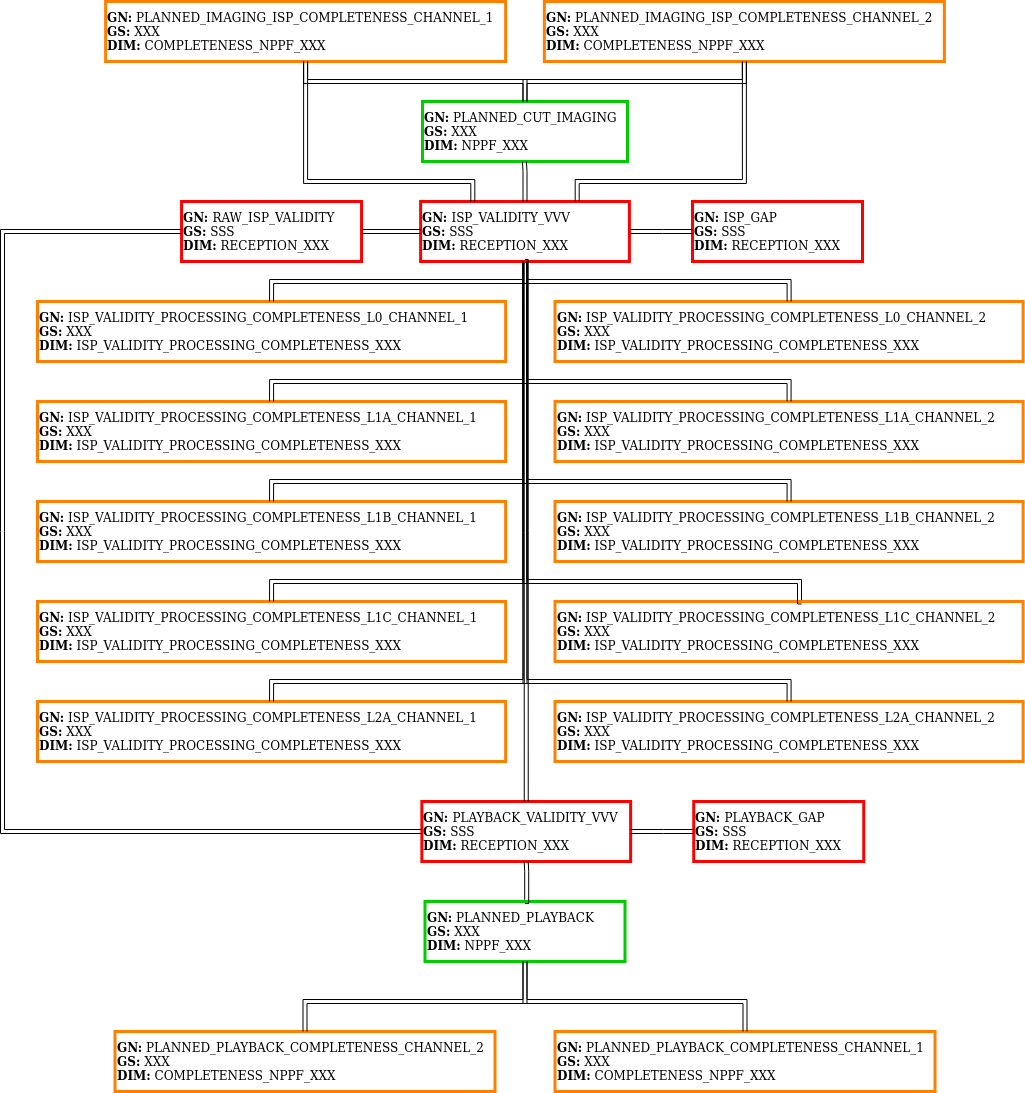
\includegraphics[width=150mm]{../fig/structure_ingestion_eisp.png}
	\caption{Structure of events inserted by the ingestion module for the REP\_PASS\_[2|5] file}
	\label{fg:structure_ingestion_eisp}
  \end{center}
\end{figure}

The table \ref{tb:description_events_ingestion_eisp} shows the description of the events inserted by the ingestion.

\begin{landscape}
\begin{longtable}{|M{0.15\linewidth}|M{0.05\linewidth}|M{0.10\linewidth}|M{0.10\linewidth}|M{0.15\linewidth}|M{0.15\linewidth}|M{0.15\linewidth}|}
\hline \textbf{Gauge name} & \textbf{Gauge system} & \textbf{DIM signature} & \textbf{Insertion mode} & \textbf{Description} & \textbf{Start} & \textbf{Stop} \\ \hline
\textbf{PLAYBACK\_VALIDITY\_VVV} & SSS & \- RECEPTION\_XXX & EVENT\_KEYS (insert) [KEY: SESSION-ID\_CHANNEL\_[1|2]] & Event for representing the \textbf{ground acquisition operation} & UTC time associated to the start of the reception & UTC time associated to the stop of the reception \\ \hline
\textbf{PLAYBACK\_GAP} & SSS & \- RECEPTION\_XXX & EVENT\_KEYS (insert) [KEY: SESSION-ID\_CHANNEL\_[1|2]] & Event for representing a \textbf{gap in the ground acquisition operation} & UTC time associated to the start of the corresponding gap in the reception & UTC time associated to the stop of the corresponding gap in the reception \\ \hline
\textbf{PLANNED\_PLAYBACK\_COMPLETENESS\_CHANNEL\_1} & XXX & \- COMPLETENESS\_NPPF\_XXX & ERASE\_and\_REPLACE\_per\_EVENT (insert) & Event for completing the \textbf{expectation of the planned playbacks through the channel 1} & Start of the reception through the channel 1 & Stop of the reception through the channel 1 \\ \hline
\textbf{PLANNED\_PLAYBACK\_COMPLETENESS\_CHANNEL\_2} & XXX & \- COMPLETENESS\_NPPF\_XXX & ERASE\_and\_REPLACE\_per\_EVENT (insert) & Event for completing the \textbf{expectation of the planned playbacks through the channel 2} & Start of the reception through the channel 2 & Stop of the reception through the channel 2 \\ \hline
\textbf{PLANNED\_IMAGING\_ISP\_COMPLETENESS\_CHANNEL\_1} & XXX & \- COMPLETENESS\_NPPF\_XXX & ERASE\_and\_REPLACE\_per\_EVENT (insert) & Event for completing the \textbf{expectation of the planned imaging sent through the channel 1} & Start of the first received scene thorugh the channel 1 of the corresponding continuous \acrshort{msi} segment & Stop of the last received scene thorugh the channel 1 of the corresponding continuous \acrshort{msi} segment \\ \hline
\textbf{PLANNED\_IMAGING\_ISP\_COMPLETENESS\_CHANNEL\_2} & XXX & \- COMPLETENESS\_NPPF\_XXX & ERASE\_and\_REPLACE\_per\_EVENT (insert) & Event for completing the \textbf{expectation of the planned imaging sent through the channel 2} & Start of the first received scene thorugh the channel 2 of the corresponding continuous \acrshort{msi} segment & Stop of the last received scene thorugh the channel 2 of the corresponding continuous \acrshort{msi} segment \\ \hline
\textbf{RAW\_ISP\_VALIDITY} & SSS & \- RECEPTION\_XXX & EVENT\_KEYS (insert) [KEY: SESSION-ID\_CHANNEL\_[1|2]] & Event for representing the \textbf{ground acquisition operation} & Start of the first received scene & Stop of the last received scene \\ \hline
\textbf{ISP\_VALIDITY} & SSS & \- RECEPTION\_XXX & EVENT\_KEYS (insert) [KEY: SESSION-ID\_CHANNEL\_[1|2]] & Event for representing the \textbf{ground acquisition operation} & Start of the first received scene of the corresponding continuous \acrshort{msi} segment & Stop of the last received scene of the corresponding continuous \acrshort{msi} segment \\ \hline
\textbf{ISP\_GAP} & SSS & \- RECEPTION\_XXX & EVENT\_KEYS (insert) [KEY: SESSION-ID\_CHANNEL\_[1|2]] & Event for representing a \textbf{gap in the ground acquisition operation} & UTC time associated to the start of the corresponding continuous gap in the received MSI & UTC time associated to the stop of the corresponding continuous gap in the received MSI \\ \hline
\textbf{ISP\_VALIDITY\_PROCESSING\_COMPLETENESS\_L0\_CHANNEL\_1} & XXX & \- COMPLETENESS\_NPPF\_XXX & ERASE\_and\_REPLACE\_per\_EVENT (insert) & Event for representing the \textbf{expectation of the processing of the planned imaging for the L0} & Start of the first received scene of the corresponding continuous \acrshort{msi} segment & Stop of the last received scene of the corresponding continuous \acrshort{msi} segment \\ \hline
\textbf{ISP\_VALIDITY\_PROCESSING\_COMPLETENESS\_L1A\_CHANNEL\_1} & XXX & \- COMPLETENESS\_NPPF\_XXX & ERASE\_and\_REPLACE\_per\_EVENT (insert) & Event for representing the \textbf{expectation of the processing of the planned imaging for the L0} & Start of the first received scene of the corresponding continuous \acrshort{msi} segment & Stop of the last received scene of the corresponding continuous \acrshort{msi} segment \\ \hline
\textbf{ISP\_VALIDITY\_PROCESSING\_COMPLETENESS\_L1B\_CHANNEL\_1} & XXX & \- COMPLETENESS\_NPPF\_XXX & ERASE\_and\_REPLACE\_per\_EVENT (insert) & Event for representing the \textbf{expectation of the processing of the planned imaging for the L0} & Start of the first received scene of the corresponding continuous \acrshort{msi} segment & Stop of the last received scene of the corresponding continuous \acrshort{msi} segment \\ \hline
\textbf{ISP\_VALIDITY\_PROCESSING\_COMPLETENESS\_L1C\_CHANNEL\_1} & XXX & \- COMPLETENESS\_NPPF\_XXX & ERASE\_and\_REPLACE\_per\_EVENT (insert) & Event for representing the \textbf{expectation of the processing of the planned imaging for the L0} & Start of the first received scene of the corresponding continuous \acrshort{msi} segment & Stop of the last received scene of the corresponding continuous \acrshort{msi} segment \\ \hline
\textbf{ISP\_VALIDITY\_PROCESSING\_COMPLETENESS\_L2A\_CHANNEL\_1} & XXX & \- COMPLETENESS\_NPPF\_XXX & ERASE\_and\_REPLACE\_per\_EVENT (insert) & Event for representing the \textbf{expectation of the processing of the planned imaging for the L0} & Start of the first received scene of the corresponding continuous \acrshort{msi} segment & Stop of the last received scene of the corresponding continuous \acrshort{msi} segment \\ \hline
\textbf{ISP\_VALIDITY\_PROCESSING\_COMPLETENESS\_L0\_CHANNEL\_2} & XXX & \- COMPLETENESS\_NPPF\_XXX & ERASE\_and\_REPLACE\_per\_EVENT (insert) & Event for representing the \textbf{expectation of the processing of the planned imaging for the L0} & Start of the first received scene of the corresponding continuous \acrshort{msi} segment & Stop of the last received scene of the corresponding continuous \acrshort{msi} segment \\ \hline
\textbf{ISP\_VALIDITY\_PROCESSING\_COMPLETENESS\_L1A\_CHANNEL\_2} & XXX & \- COMPLETENESS\_NPPF\_XXX & ERASE\_and\_REPLACE\_per\_EVENT (insert) & Event for representing the \textbf{expectation of the processing of the planned imaging for the L0} & Start of the first received scene of the corresponding continuous \acrshort{msi} segment & Stop of the last received scene of the corresponding continuous \acrshort{msi} segment \\ \hline
\textbf{ISP\_VALIDITY\_PROCESSING\_COMPLETENESS\_L1B\_CHANNEL\_2} & XXX & \- COMPLETENESS\_NPPF\_XXX & ERASE\_and\_REPLACE\_per\_EVENT (insert) & Event for representing the \textbf{expectation of the processing of the planned imaging for the L0} & Start of the first received scene of the corresponding continuous \acrshort{msi} segment & Stop of the last received scene of the corresponding continuous \acrshort{msi} segment \\ \hline
\textbf{ISP\_VALIDITY\_PROCESSING\_COMPLETENESS\_L1C\_CHANNEL\_2} & XXX & \- COMPLETENESS\_NPPF\_XXX & ERASE\_and\_REPLACE\_per\_EVENT (insert) & Event for representing the \textbf{expectation of the processing of the planned imaging for the L0} & Start of the first received scene of the corresponding continuous \acrshort{msi} segment & Stop of the last received scene of the corresponding continuous \acrshort{msi} segment \\ \hline
\textbf{ISP\_VALIDITY\_PROCESSING\_COMPLETENESS\_L2A\_CHANNEL\_2} & XXX & \- COMPLETENESS\_NPPF\_XXX & ERASE\_and\_REPLACE\_per\_EVENT (insert) & Event for representing the \textbf{expectation of the processing of the planned imaging for the L0} & Start of the first received scene of the corresponding continuous \acrshort{msi} segment & Stop of the last received scene of the corresponding continuous \acrshort{msi} segment \\ \hline
\caption{Table describing the events associated to the ingestion}
\label{tb:description_events_ingestion_eisp}
\end{longtable}
\end{landscape}


% Ingestion of the REP_OPDPC
% \section{Ingestion module for the REP\_OPDPC file}

This sections describes the ingestion module for inserting the \acrshort{dpc} processing analysis.

The associated ingestion processor is:

\begin{itemize} 

\item \textbf{s2boa.ingestions.ingestion\_dpc.ingestion\_dpc}
  
\end{itemize}

This module uses the following \acrshort{dim} signatures:

\begin{itemize} 

\item \textbf{PROCESSING\_XXX}: data corresponding to the processing analysis.

\item \textbf{COMPLETENESS\_NPPF\_XXX}: data corresponding to the definition of planning completeness used for analysis.

\item \textbf{ISP\_VALIDITY\_PROCESSING\_COMPLETENESS\_XXX}: data corresponding to the definition of \acrshort{isp} processing completeness used for analysis.

\item \textbf{INDEXING\_XXX}: data corresponding to the indexing analysis of products.

\item \textbf{ARCHIVING}: data corresponding to the archiving analysis of products.

\item \textbf{CATALOGING}: data corresponding to the cataloging analysis of products.

\item \textbf{LONG\_TERM\_ARCHIVING}: data corresponding to the cataloging analysis of products.

\end{itemize}

Where XXX is the corresponding satellite id.

The figure \ref{fg:structure_ingestion_dpc_events} shows a simplified diagram of the structure of events inserted (associated structure of values not included for simplicity).

\begin{figure}[H]
  \begin{center}
	\centering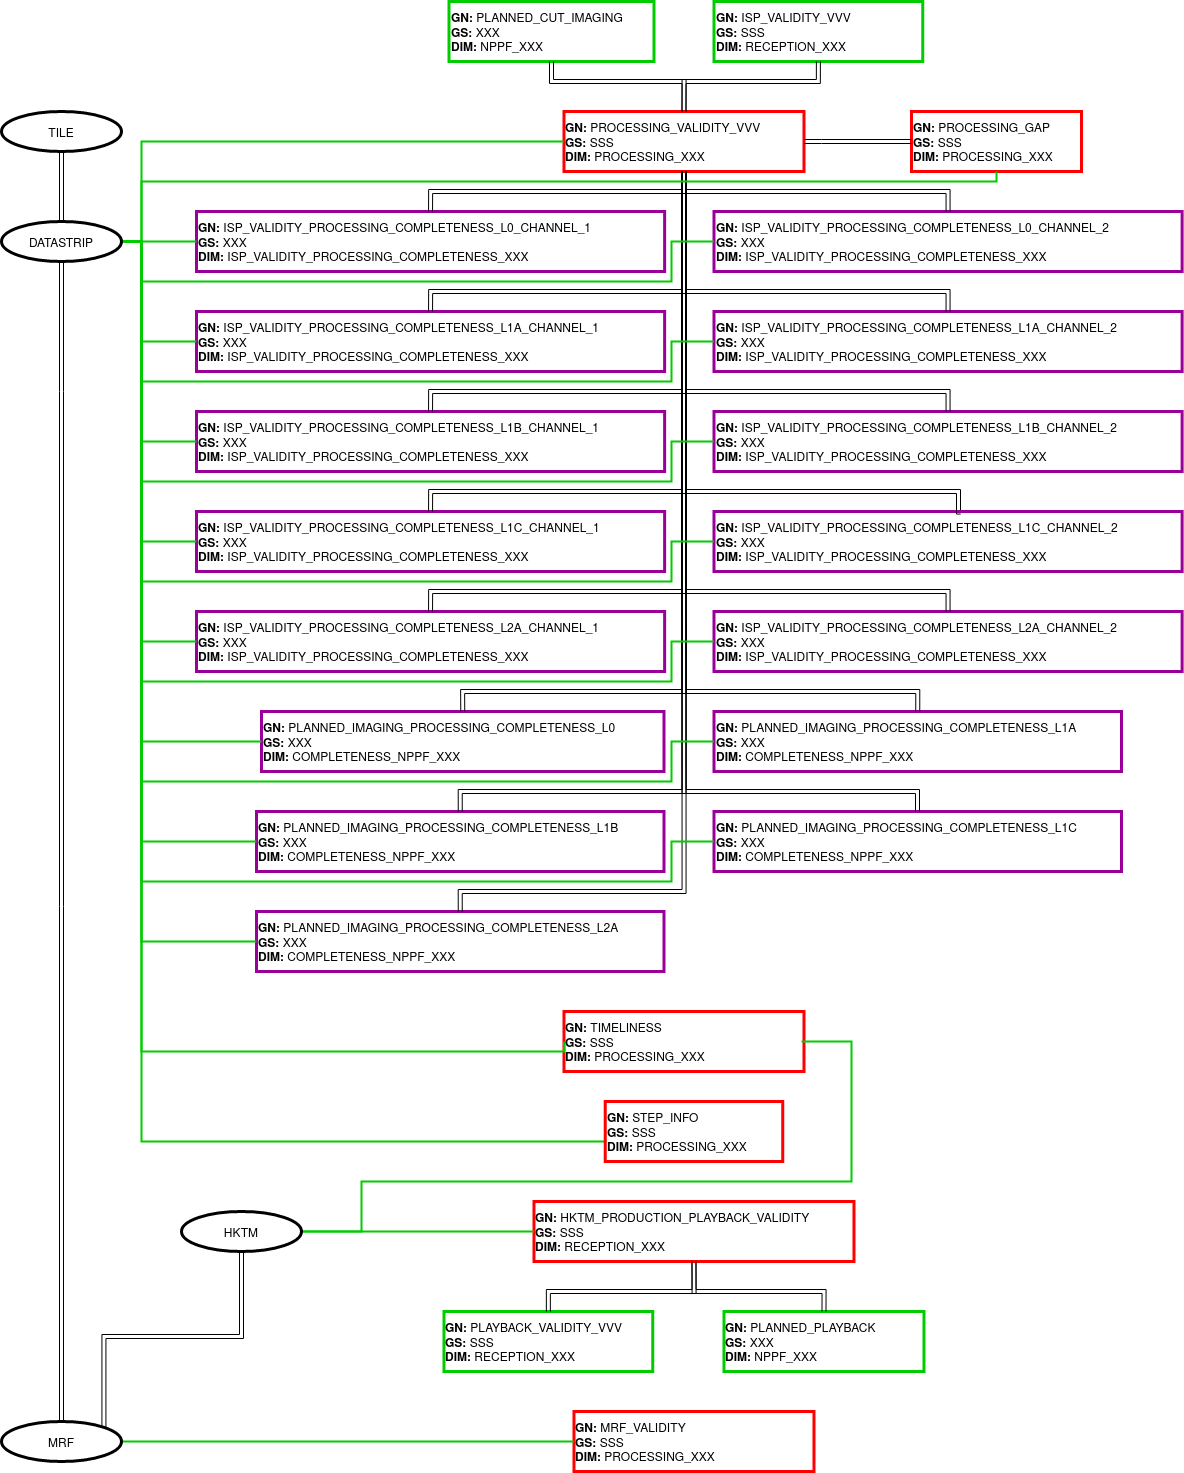
\includegraphics[width=150mm]{../fig/structure_ingestion_dpc_events.png}
	\caption{Structure of events inserted by the ingestion module for the REP\_OPDPC file}
	\label{fg:structure_ingestion_dpc_events}
  \end{center}
\end{figure}

The table \ref{tb:description_events_ingestion_dpc} shows the description of the events inserted by the ingestion.

\begin{landscape}
\begin{longtable}{|M{0.15\linewidth}|M{0.05\linewidth}|M{0.10\linewidth}|M{0.10\linewidth}|M{0.15\linewidth}|M{0.15\linewidth}|M{0.15\linewidth}|}
\hline \textbf{Gauge name} & \textbf{Gauge system} & \textbf{DIM signature} & \textbf{Insertion mode} & \textbf{Description} & \textbf{Start} & \textbf{Stop} \\ \hline
\textbf{PLAYBACK\_VALIDITY\_VVV} & SSS & \- RECEPTION\_XXX & EVENT\_KEYS (insert) & Event for representing the \textbf{ground acquisition operation} & UTC time associated to the start of the reception & UTC time associated to the stop of the reception \\ \hline
\textbf{PLAYBACK\_GAP} & SSS & \- RECEPTION\_XXX & EVENT\_KEYS (insert) & Event for representing a \textbf{gap in the ground acquisition operation} & UTC time associated to the start of the corresponding gap in the reception & UTC time associated to the stop of the corresponding gap in the reception \\ \hline
\textbf{PLANNED\_PLAYBACK\_COMPLETENESS\_CHANNEL\_1} & XXX & \- COMPLETENESS\_NPPF\_XXX & ERASE\_and\_REPLACE\_per\_EVENT (insert) & Event for completing the \textbf{expectation of the planned playbacks through the channel 1} & Start of the reception through the channel 1 & Stop of the reception through the channel 1 \\ \hline
\textbf{PLANNED\_PLAYBACK\_COMPLETENESS\_CHANNEL\_2} & XXX & \- COMPLETENESS\_NPPF\_XXX & ERASE\_and\_REPLACE\_per\_EVENT (insert) & Event for completing the \textbf{expectation of the planned playbacks through the channel 2} & Start of the reception through the channel 2 & Stop of the reception through the channel 2 \\ \hline
\textbf{PLANNED\_IMAGING\_ISP\_COMPLETENESS\_CHANNEL\_1} & XXX & \- COMPLETENESS\_NPPF\_XXX & ERASE\_and\_REPLACE\_per\_EVENT (insert) & Event for completing the \textbf{expectation of the planned imaging sent through the channel 1} & Start of the first received scene thorugh the channel 1 of the corresponding continuous \acrshort{msi} segment & Stop of the last received scene thorugh the channel 1 of the corresponding continuous \acrshort{msi} segment \\ \hline
\textbf{PLANNED\_IMAGING\_ISP\_COMPLETENESS\_CHANNEL\_2} & XXX & \- COMPLETENESS\_NPPF\_XXX & ERASE\_and\_REPLACE\_per\_EVENT (insert) & Event for completing the \textbf{expectation of the planned imaging sent through the channel 2} & Start of the first received scene thorugh the channel 2 of the corresponding continuous \acrshort{msi} segment & Stop of the last received scene thorugh the channel 2 of the corresponding continuous \acrshort{msi} segment \\ \hline
\textbf{RAW\_ISP\_VALIDITY} & SSS & \- RECEPTION\_XXX & EVENT\_KEYS (insert) & Event for representing the \textbf{ground acquisition operation} & Start of the first received scene & Stop of the last received scene \\ \hline
\textbf{ISP\_VALIDITY} & SSS & \- RECEPTION\_XXX & EVENT\_KEYS (insert) & Event for representing the \textbf{ground acquisition operation} & Start of the first received scene of the corresponding continuous \acrshort{msi} segment & Stop of the last received scene of the corresponding continuous \acrshort{msi} segment \\ \hline
\textbf{ISP\_GAP} & SSS & \- RECEPTION\_XXX & EVENT\_KEYS (insert) & Event for representing a \textbf{gap in the ground acquisition operation} & UTC time associated to the start of the corresponding continuous gap in the received MSI & UTC time associated to the stop of the corresponding continuous gap in the received MSI \\ \hline
\textbf{PLAYBACK\_ISP\_DISTRIBUTION\_STATUS\_CHANNEL\_1} & SSS & \- RECEPTION\_XXX & EVENT\_KEYS (insert) & Event for representing a \textbf{gap in the ground acquisition operation} & UTC time associated to the start of the \acrshort{msi} reception & UTC time associated to the stop of the \acrshort{msi} reception \\ \hline
\textbf{PLAYBACK\_ISP\_DISTRIBUTION\_STATUS\_CHANNEL\_2} & SSS & \- RECEPTION\_XXX & EVENT\_KEYS (insert) & Event for representing a \textbf{gap in the ground acquisition operation} & UTC time associated to the start of the \acrshort{msi} reception & UTC time associated to the stop of the \acrshort{msi} reception \\ \hline
\textbf{PLAYBACK\_HKTM\_DISTRIBUTION\_STATUS\_CHANNEL\_1} & SSS & \- RECEPTION\_XXX & EVENT\_KEYS (insert) & Event for representing a \textbf{gap in the ground acquisition operation} & UTC time associated to the start of the corresponding gap in the \acrshort{hktm} reception & UTC time associated to the stop of the corresponding gap in the \acrshort{hktm} reception \\ \hline
\textbf{PLAYBACK\_HKTM\_DISTRIBUTION\_STATUS\_CHANNEL\_2} & SSS & \- RECEPTION\_XXX & EVENT\_KEYS (insert) & Event for representing a \textbf{gap in the ground acquisition operation} & UTC time associated to the start of the corresponding gap in the \acrshort{hktm} reception & UTC time associated to the stop of the corresponding gap in the \acrshort{hktm} reception \\ \hline
\textbf{DFEP\_ACQUISITION\_VALIDITY} & SSS & \- RECEPTION\_XXX & EVENT\_KEYS (insert) & Event for representing a \textbf{gap in the ground acquisition operation} & UTC time associated to the validity start of the received file & UTC time associated to the validity stop of the received file \\ \hline
\textbf{ISP\_VALIDITY\_PROCESSING\_COMPLETENESS\_L0\_CHANNEL\_1} & XXX & \- COMPLETENESS\_NPPF\_XXX & ERASE\_and\_REPLACE\_per\_EVENT (insert) & Event for representing the \textbf{expectation of the processing of the planned imaging for the L0} & Start of the first received scene of the corresponding continuous \acrshort{msi} segment & Stop of the last received scene of the corresponding continuous \acrshort{msi} segment \\ \hline
\textbf{ISP\_VALIDITY\_PROCESSING\_COMPLETENESS\_L1A\_CHANNEL\_1} & XXX & \- COMPLETENESS\_NPPF\_XXX & ERASE\_and\_REPLACE\_per\_EVENT (insert) & Event for representing the \textbf{expectation of the processing of the planned imaging for the L0} & Start of the first received scene of the corresponding continuous \acrshort{msi} segment & Stop of the last received scene of the corresponding continuous \acrshort{msi} segment \\ \hline
\textbf{ISP\_VALIDITY\_PROCESSING\_COMPLETENESS\_L1B\_CHANNEL\_1} & XXX & \- COMPLETENESS\_NPPF\_XXX & ERASE\_and\_REPLACE\_per\_EVENT (insert) & Event for representing the \textbf{expectation of the processing of the planned imaging for the L0} & Start of the first received scene of the corresponding continuous \acrshort{msi} segment & Stop of the last received scene of the corresponding continuous \acrshort{msi} segment \\ \hline
\textbf{ISP\_VALIDITY\_PROCESSING\_COMPLETENESS\_L1C\_CHANNEL\_1} & XXX & \- COMPLETENESS\_NPPF\_XXX & ERASE\_and\_REPLACE\_per\_EVENT (insert) & Event for representing the \textbf{expectation of the processing of the planned imaging for the L0} & Start of the first received scene of the corresponding continuous \acrshort{msi} segment & Stop of the last received scene of the corresponding continuous \acrshort{msi} segment \\ \hline
\textbf{ISP\_VALIDITY\_PROCESSING\_COMPLETENESS\_L2A\_CHANNEL\_1} & XXX & \- COMPLETENESS\_NPPF\_XXX & ERASE\_and\_REPLACE\_per\_EVENT (insert) & Event for representing the \textbf{expectation of the processing of the planned imaging for the L0} & Start of the first received scene of the corresponding continuous \acrshort{msi} segment & Stop of the last received scene of the corresponding continuous \acrshort{msi} segment \\ \hline
\textbf{ISP\_VALIDITY\_PROCESSING\_COMPLETENESS\_L0\_CHANNEL\_2} & XXX & \- COMPLETENESS\_NPPF\_XXX & ERASE\_and\_REPLACE\_per\_EVENT (insert) & Event for representing the \textbf{expectation of the processing of the planned imaging for the L0} & Start of the first received scene of the corresponding continuous \acrshort{msi} segment & Stop of the last received scene of the corresponding continuous \acrshort{msi} segment \\ \hline
\textbf{ISP\_VALIDITY\_PROCESSING\_COMPLETENESS\_L1A\_CHANNEL\_2} & XXX & \- COMPLETENESS\_NPPF\_XXX & ERASE\_and\_REPLACE\_per\_EVENT (insert) & Event for representing the \textbf{expectation of the processing of the planned imaging for the L0} & Start of the first received scene of the corresponding continuous \acrshort{msi} segment & Stop of the last received scene of the corresponding continuous \acrshort{msi} segment \\ \hline
\textbf{ISP\_VALIDITY\_PROCESSING\_COMPLETENESS\_L1B\_CHANNEL\_2} & XXX & \- COMPLETENESS\_NPPF\_XXX & ERASE\_and\_REPLACE\_per\_EVENT (insert) & Event for representing the \textbf{expectation of the processing of the planned imaging for the L0} & Start of the first received scene of the corresponding continuous \acrshort{msi} segment & Stop of the last received scene of the corresponding continuous \acrshort{msi} segment \\ \hline
\textbf{ISP\_VALIDITY\_PROCESSING\_COMPLETENESS\_L1C\_CHANNEL\_2} & XXX & \- COMPLETENESS\_NPPF\_XXX & ERASE\_and\_REPLACE\_per\_EVENT (insert) & Event for representing the \textbf{expectation of the processing of the planned imaging for the L0} & Start of the first received scene of the corresponding continuous \acrshort{msi} segment & Stop of the last received scene of the corresponding continuous \acrshort{msi} segment \\ \hline
\textbf{ISP\_VALIDITY\_PROCESSING\_COMPLETENESS\_L2A\_CHANNEL\_2} & XXX & \- COMPLETENESS\_NPPF\_XXX & ERASE\_and\_REPLACE\_per\_EVENT (insert) & Event for representing the \textbf{expectation of the processing of the planned imaging for the L0} & Start of the first received scene of the corresponding continuous \acrshort{msi} segment & Stop of the last received scene of the corresponding continuous \acrshort{msi} segment \\ \hline
\caption{Table describing the events associated to the ingestion}
\label{tb:description_events_ingestion_dpc}
\end{longtable}
\end{landscape}

The figure \ref{fg:structure_ingestion_dpc_annotations} shows a simplified diagram of the structure of annotations inserted (associated structure of values not included for simplicity).

\begin{figure}[H]
  \begin{center}
	\centering\includegraphics[width=150mm]{../fig/structure_ingestion_dpc_annotations.png}
	\caption{Structure of annotations inserted by the ingestion module for the REP\_OPDPC file}
	\label{fg:structure_ingestion_dpc_annotations}
  \end{center}
\end{figure}


% Ingestion of the OPHKTM
\section{Ingestion module for the OPHKTM file}

This sections describes the ingestion module for inserting the production information of the package, which contains the housekeeping telemetry received from the satellite, generated by \acrshort{pdgs} to be sent to \acrshort{fos}.

The associated ingestion processors are:

\begin{itemize} 

\item \textbf{s2boa.ingestions.ingestion\_ophktm.ingestion\_ophktm}
  
\end{itemize}

This module uses the following \acrshort{dim} signatures:

\begin{itemize} 

\item \textbf{HKTM\_PRODUCTION\_VGS}: production information of the package, which contains the housekeeping telemetry received from the satellite, generated by \acrshort{pdgs} to be sent to \acrshort{fos}.
  
\end{itemize}

The table \ref{tb:description_explicit_reference_ingestion_ophktm} shows the description of the explicit references inserted by the ingestion.

\begin{longtable}{|M{0.3\linewidth}|M{0.55\linewidth}|}
\hline \textbf{Reference} & \textbf{Description} \\ \hline
\textbf{HKTM PRODUCT\_ID} & Identifier of the package generated by \acrshort{pdgs} containing the telemetry to be sent to \acrshort{fos} \\ \hline
\caption{Table describing the explicit reference associated to the ingestion}
\label{tb:description_explicit_reference_ingestion_ophktm}
\end{longtable}

The figure \ref{fg:structure_ingestion_ophktm_events} shows a simplified diagram of the structure of events inserted (associated structure of values not included for simplicity).

\begin{figure}[H]
  \begin{center}
	\centering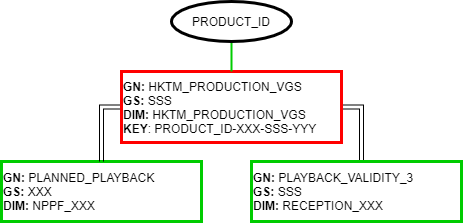
\includegraphics[scale=0.7]{../fig/structure_ingestion_ophktm_events.png}
	\caption{Structure of events inserted by the ingestion module for the OPHKTM file}
	\label{fg:structure_ingestion_ophktm_events}
  \end{center}
\end{figure}

Where XXX is the corresponding satellite id, SSS is the station and YYY is the orbit number.

The table \ref{tb:description_events_ingestion_ophktm} shows the description of the events inserted by the ingestion.

\begin{landscape}
\begin{longtable}{|M{0.15\linewidth}|M{0.05\linewidth}|M{0.10\linewidth}|M{0.10\linewidth}|M{0.15\linewidth}|M{0.15\linewidth}|M{0.15\linewidth}|}
\hline \textbf{Gauge name} & \textbf{Gauge system} & \textbf{DIM signature} & \textbf{Insertion mode} & \textbf{Description} & \textbf{Start} & \textbf{Stop} \\ \hline
\textbf{HKTM\_PRODUCTION\_VGS} & XXX & HKTM\_PRODUCTION\_VGS & EVENT\_KEYS (insert) [KEY: PRODUCT\_ID-XXX-SSS-YYY] & Event for representing the \textbf{generation of the HKTM product} & UTC value inside the generation\_date node & UTC value inside the generation\_date node  \\ \hline
\caption{Table describing the events associated to the ingestion}
\label{tb:description_events_ingestion_ophktm}
\end{longtable}
\end{landscape}

The figure \ref{fg:structure_ingestion_ophktm_annotations} shows a simplified diagram of the structure of annotations inserted (associated structure of values not included for simplicity).

\begin{figure}[H]
  \begin{center}
	\centering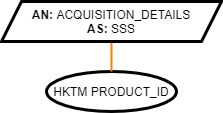
\includegraphics[scale=0.7]{../fig/structure_ingestion_ophktm_annotations.png}
	\caption{Structure of annotations inserted by the ingestion module for the OPHKTM file}
	\label{fg:structure_ingestion_ophktm_annotations}
  \end{center}
\end{figure}

Where SSS is the station.

The table \ref{tb:description_annotations_ingestion_ophktm} shows the description of the annotations inserted by the ingestion.

\begin{longtable}{|M{0.2\linewidth}|M{0.15\linewidth}|M{0.15\linewidth}|M{0.10\linewidth}|M{0.25\linewidth}|}
\hline \textbf{Annotation name} & \textbf{Annotation system} & \textbf{DIM signature} & \textbf{Insertion mode} & \textbf{Description} \\ \hline
\textbf{ACQUISITION\_DETAILS} & SSS & HKTM\_PRODUCTION\_VGS & SIMPLE\_UPDATE (insert) & Annotation for representing the \textbf{acquisition details for the generated HKTM package} \\ \hline
\caption{Table describing the annotations associated to the ingestion}
\label{tb:description_annotations_ingestion_ophktm}
\end{longtable}




%Ingestion of TLM_REQ_B 
\section{Ingestion module for the TLM\_REQ\_B\ files}

This section describes the ingestion module for inserting the telemetry files containing the memory information of the satellite.
The associated ingestion processor is 

\begin{itemize}
    \item \textbf{s2boa.ingestions.ingestion\_tlm\_req\_b.ingestion\_tlm\_req\_b}
\end{itemize}

This module uses the folowing \acrshort{dim} signatures:
\begin{itemize}
    \item \textbf{MEMORY\_EVOLUTION\_XXX}: data containing the evolution of the memory in the different storages (NOMINAL, NRT) for the two channels as well as the last replayed scene to ground for the two channels.
\end{itemize}

Where XXX is the corresponding satellite id.

The figure \ref{fig:structure_ingestion_tlm_req_b} shows a simplified diagram of the structure of events inserted (associated structure of values not included for simplicity).

\begin{figure}[H]
  \begin{center}
	\centering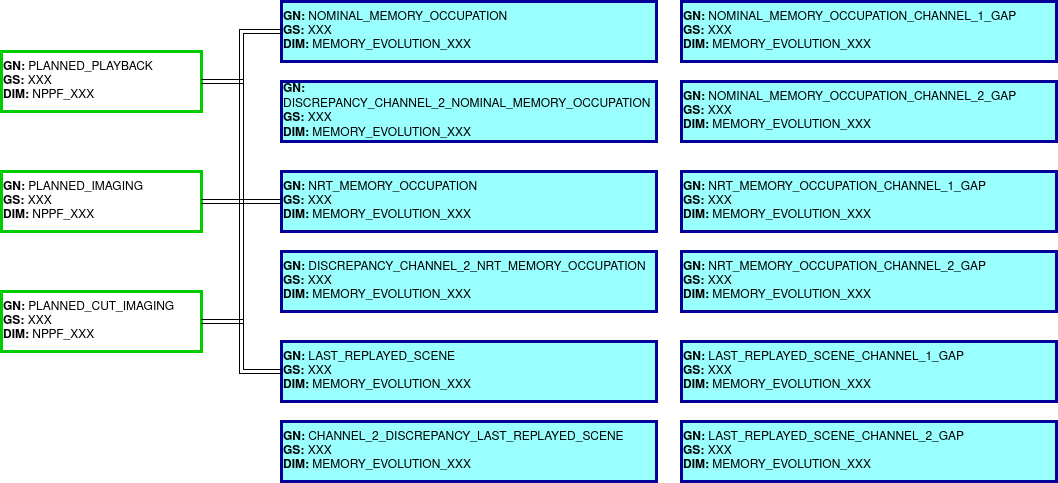
\includegraphics[width=170mm]{../fig/structure_ingestion_tlm_req_b.png}
	\caption{Structure of events inserted by the ingestion module for the TLM\_REQ\_B file}
	\label{fig:structure_ingestion_tlm_req_b}
  \end{center}
\end{figure}

The table \ref{tb:description_events_ingestion_tlm_req_b} shows the description of the events inserted by the ingestion module.
\begin{landscape}
    \begin{longtable}{|M{0.15\linewidth}|M{0.05\linewidth}|M{0.10\linewidth}|M{0.10\linewidth}|M{0.2\linewidth}|M{0.125\linewidth}|M{0.125\linewidth}|}
    \hline \textbf{Gauge name} & \textbf{Gauge system} & \textbf{DIM signature} & \textbf{Insertion mode} & \textbf{Description} & \textbf{Start} & \textbf{Stop} \\ \hline
    \textbf{NOMINAL\_MEMORY\_OCCUPATION} & XXX & \- MEMORY\_EVOLUTION\_XXX & INSERT\_and\_ERASE (insert\_and\_erase) & Event for representing the \textbf{NOMINAL memory evolution} taking as reference the values for channel 1& UTC time associated to a new engineering\_value & UTC time associated to the last instance of the same enineering\_value \\ \hline
    \textbf{DISCREPANCY\_CHANNEL\_2\_NOMINAL\_MEMORY\_OCCUPATION} & XXX & \- MEMORY\_EVOLUTION\_XXX & INSERT\_and\_ERASE (insert\_and\_erase) & Event for representing the \textbf{discrepancy between the NOMINAL memory occupation of Channel 1 and the NOMINAL memory occupation of Channel 2} & UTC time associated to the discrepancy & UTC time associated to the discrepancy \\ \hline
    \textbf{NRT\_MEMORY\_OCCUPATION} & XXX & \- MEMORY\_EVOLUTION\_XXX & INSERT\_and\_ERASE (insert\_and\_erase) & Event for representing the \textbf{NRT memory evolution} taking as reference the values for channel 1 & UTC time associated to a new engineering\_value & UTC time associated to the last instance of the same enineering\_value  \\ \hline
    \textbf{DISCREPANCY\_CHANNEL\_2\_NRT\_MEMORY\_OCCUPATION} & XXX & \- MEMORY\_EVOLUTION\_XXX & INSERT\_and\_ERASE (insert\_and\_erase) & Event for representing the \textbf{discrepancy between the NRT memory occupation of Channel 1 and NRT memory occupation of Channel 2} & UTC time associated to the discrepancy & UTC time associated to the discrepancy \\ \hline
    \textbf{LAST\_REPLAYED\_SCENE} & XXX & \- MEMORY\_EVOLUTION\_XXX & INSERT\_and\_ERASE (insert\_and\_erase) & Event for representing the \textbf{last replayed scene} taking as reference the values for channel 1 & UTC time associated to a new engineering\_value & UTC time associated to the last instance of the same enineering\_value  \\ \hline
    \textbf{DISCREPANCY\_CHANNEL\_2\_LAST\_REPLAYED\_SCENE} & XXX & \- MEMORY\_EVOLUTION\_XXX & INSERT\_and\_ERASE (insert\_and\_erase) & Event for representing the \textbf{discrepancy between the last replayed scene of Channel 1 and the last replayed scene of Channel 2} & UTC time associated to the discrepancy & UTC time associated to the discrepancy  \\ \hline
    \textbf{NOMINAL\_MEMORY\_OCCUPATION\_CHANNEL\_1\_GAP} & XXX & \- MEMORY\_EVOLUTION\_XXX & INSERT\_and\_ERASE (insert\_and\_erase) & Event for representing the \textbf{gaps in the NOMINAL memory occupation of Channel 1} of more than 6 seconds & UTC time associated to the beginning of the gap & UTC time associated to the end of the gap  \\ \hline
    \textbf{NOMINAL\_MEMORY\_OCCUPATION\_CHANNEL\_2\_GAP} & XXX & \- MEMORY\_EVOLUTION\_XXX & INSERT\_and\_ERASE (insert\_and\_erase) & Event for representing the \textbf{gaps in the NOMINAL memory occupation of Channel 2} of more than 6 seconds& UTC time associated to the beginning of the gap & UTC time associated to the end of the gap  \\ \hline
    \textbf{NRT\_MEMORY\_OCCUPATION\_CHANNEL\_1\_GAP} & XXX & \- MEMORY\_EVOLUTION\_XXX & INSERT\_and\_ERASE (insert\_and\_erase) & Event for representing the \textbf{gaps in the NRT memory occupation of Channel 1} of more than 6 seconds& UTC time associated to the beginning of the gap & UTC time associated to the end of the gap  \\ \hline
    \textbf{NRT\_MEMORY\_OCCUPATION\_CHANNEL\_2\_GAP} & XXX & \- MEMORY\_EVOLUTION\_XXX & INSERT\_and\_ERASE (insert\_and\_erase) & Event for representing the \textbf{gaps in the NRT memory occupation of Channel 2} of more than 6 seconds& UTC time associated to the beginning of the gap & UTC time associated to the end of the gap  \\ \hline
    \textbf{LAST\_REPLAYED\_SCENE\_CHANNEL\_1\_GAP} & XXX & \- MEMORY\_EVOLUTION\_XXX & INSERT\_and\_ERASE (insert\_and\_erase) & Event for representing the \textbf{gaps in the last replayed scene data of Channel 1} of more than 6 seconds& UTC time associated to the beginning of the gap & UTC time associated to the end of the gap  \\ \hline
    \textbf{LAST\_REPLAYED\_SCENE\_CHANNEL\_2\_GAP} & XXX & \- MEMORY\_EVOLUTION\_XXX & INSERT\_and\_ERASE (insert\_and\_erase) & Event for representing the \textbf{gaps in the last replayed scene data of Channel 2} of more than 6 seconds& UTC time associated to the beginning of the gap & UTC time associated to the end of the gap  \\ \hline
    \caption{Table describing the events associated to the ingestion}
    \label{tb:description_events_ingestion_tlm_req_b}
    \end{longtable}
    \end{landscape}
